         \chapter{Trigonometry}
    \setcounter{figure}{1}
    \setcounter{subfigure}{1}
    \label{fbcda86bdf0258b6e91dcea5caee5b76}
%          \section{ Introduction and key concepts}
%     \nopagebreak
%             \label{m39405} $ \hspace{-5pt}\begin{array}{cccccccccccc}   \end{array} $ \hspace{2 pt}\raisebox{-5 pt}{
\includegraphics[width=0.5cm]{col11306.imgs/summary_www.png}} {(section shortcode: MG10100 )} \par 
%     
%     
%     
%   
%     \label{m39405*cid2}
%             \subsection{ Introduction}
%             \nopagebreak
%             
      \label{m39405*id77510}In geometry we learn about how the sides of polygons relate to the angles in the polygons, but we have not learned how to calculate an angle if we only know the lengths of the sides. Trigonometry (pronounced: trig-oh-nom-eh-tree) deals with the relationship between the angles and the sides of a right-angled triangle. We will learn about trigonometric functions, which form the basis of trigonometry.\par 
\label{m39405*secfhsst!!!underscore!!!id65}
%             \subsubsection{  Investigation : History of Trigonometry }
%             \nopagebreak
%             
%       \label{m39405*id77524}Work in pairs or groups and investigate the history of the foundation of trigonometry. Describe the various stages of development and how the following cultures used trigonometry to improve their lives.\par 
%       \label{m39405*id77870}The works of the following people or cultures can be investigated:\par 
%       \label{m39405*id77873}\begin{enumerate}[noitemsep, label=\textbf{\arabic*}. ] 
%             \label{m39405*uid1}\item Cultures
% \label{m39405*id77887}\begin{enumerate}[noitemsep, label=\textbf{\alph*}. ] 
%             \label{m39405*uid2}\item Ancient Egyptians
% \label{m39405*uid3}\item Mesopotamians
% \label{m39405*uid4}\item Ancient Indians of the Indus Valley
% \end{enumerate}
%         \label{m39405*uid5}\item People
% \label{m39405*id77937}\begin{enumerate}[noitemsep, label=\textbf{\alph*}. ] 
%             \label{m39405*uid6}\item Lagadha (circa 1350-1200 BC)
% \label{m39405*uid7}\item Hipparchus (circa 150 BC)
% \label{m39405*uid8}\item Ptolemy (circa 100)
% \label{m39405*uid9}\item Aryabhata (circa 499)
% \label{m39405*uid10}\item Omar Khayyam (1048-1131)
% \label{m39405*uid11}\item Bhaskara (circa 1150)
% \label{m39405*uid12}\item Nasir al-Din (13th century)
% \label{m39405*uid13}\item al-Kashi and Ulugh Beg (14th century)
% \label{m39405*uid14}\item Bartholemaeus Pitiscus (1595)
% \end{enumerate}
%         \end{enumerate}
%         
%       
% 
% \label{m39405*notfhsst!!!underscore!!!id88}
% \begin{tabular}{cc}
% 	\hspace*{-50pt}\raisebox{-8 mm}{\hspace{-0.2in}
\includegraphics[width=0.75in]{col11306.imgs/psfact2.png} } & 
% 
% 	\begin{minipage}{0.85\textwidth}
% 	\begin{note}
%       {note: }
%       \label{m39405*id78058}You should be familiar with the idea of measuring angles from geometry but have you ever stopped to think why there are 360 degrees in a circle? The reason is purely historical. There are 360 degrees in a circle because the ancient Babylonians had a number system with base 60. A base is the number at which you add another digit when you count. The number system that we use everyday is called the decimal system (the base is 10), but computers use the binary system (the base is 2). $360=6\ensuremath{\times}60$ so for them it made sense to have 360 degrees in a circle.\par 
% 
% 	\end{note}
% 	\end{minipage}
% 	\end{tabular}
% 	\par
    \label{m39405*cid3}
            \section{ Where Trigonometry is Used}
            \nopagebreak
      \label{m39405*id78100}There are many applications of trigonometry. Of particular value is the technique of triangulation, which is used in astronomy to measure the distance to nearby stars, in geography to measure distances between landmarks, and in satellite navigation systems. GPSs (global positioning systems) would not be possible without trigonometry. Other fields which make use of trigonometry include astronomy (and hence navigation, on the oceans, in aircraft, and in space), music theory, acoustics, optics, analysis of financial markets, electronics, probability theory, statistics, biology, medical imaging (CAT scans and ultrasound), pharmacy, chemistry, number theory (and hence cryptology), seismology, meteorology, oceanography, many physical sciences, land surveying and geodesy, architecture, phonetics, economics, electrical engineering, mechanical engineering, civil engineering, computer graphics, cartography, crystallography and game development.\par 
% \label{m39405*secfhsst!!!underscore!!!id95}
%             \subsection{  Discussion : Uses of Trigonometry }
%             \nopagebreak
%             
%       \label{m39405*id78126}Select one of the fields that uses trigonometry from the list given above and write a 1-page report describing \textsl{how} trigonometry is used in the field that you chose. \par 
    \label{m39405*cid4}
            \section{ Similarity of Triangles}
            \nopagebreak
      \label{m39405*id78153}If $▵ABC$ is similar to $▵DEF$, then this is written as:\par 
      \label{m39405*id78186}\nopagebreak\noindent{}
    \begin{equation}
    ▵ABC|||▵DEF\tag{14.1}
      \end{equation}
      \label{m39405*id78214}
    \setcounter{subfigure}{0}
	\begin{figure}[H] % horizontal\label{m39405*id78218}
    \begin{center}
    \label{m39405*id78218!!!underscore!!!media}\label{m39405*id78218!!!underscore!!!printimage}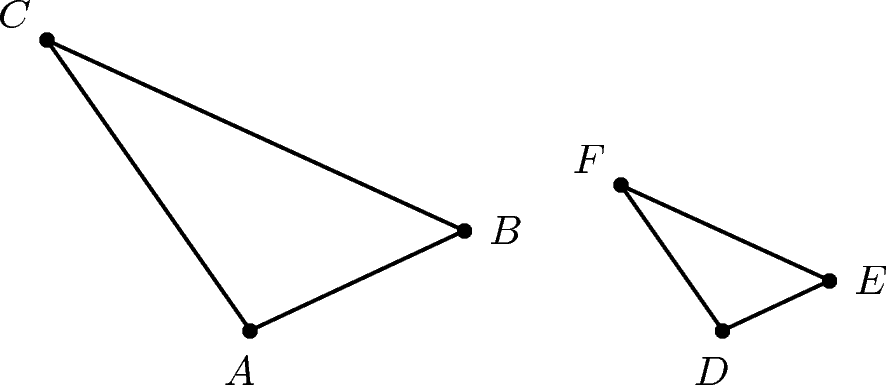
\includegraphics{col11306.imgs/m39405_MG10C15_001.png} % m39405;MG10C15\_001.png;;;6.0;8.5;
      \vspace{2pt}
    \vspace{.1in}
    \end{center}
 \end{figure}       
      \par 
      \label{m39405*id78224}Then, it is possible to deduce ratios between corresponding sides of the two triangles, such as the following:\par 
      \label{m39405*id78228}\nopagebreak\noindent{}
        
    \begin{equation}
    \begin{array}{ccc}\hfill \frac{AB}{BC}& =& \frac{DE}{EF}\hfill \\ \hfill \frac{AB}{AC}& =& \frac{DE}{DF}\hfill \\ \hfill \frac{AC}{BC}& =& \frac{DF}{EF}\hfill \\ \hfill \frac{AB}{DE}& =& \frac{BC}{EF}=\frac{AC}{DF}\hfill \end{array}\tag{14.2}
      \end{equation}
      \label{m39405*id78401}The most important fact about similar triangles $ABC$ and $DEF$ is that the angle at vertex A is equal to the angle at vertex D, the angle at B is equal to the angle at E, and the angle at C is equal to the angle at F.\par 
      \label{m39405*id78434}\nopagebreak\noindent{}
        
    \begin{equation}
    \begin{array}{ccc}\hfill \angle A& =& \angle D\hfill \\ \hfill \angle B& =& \angle E\hfill \\ \hfill \angle C& =& \angle F\hfill \end{array}\tag{14.3}
      \end{equation}
\label{m39405*secfhsst!!!underscore!!!id319}
            \subsection{  Investigation : Ratios of Similar Triangles }
            \nopagebreak
      \label{m39405*id78516}In your exercise book, draw three similar triangles of different sizes, but each with $\hat{A}={30}^{\circ }$; $\hat{B}={90}^{\circ }$ and $\hat{C}={60}^{\circ }$. Measure angles and lengths very accurately in order to fill in the table below (round answers to one decimal place).\par 
      \label{m39405*id78597}
    \setcounter{subfigure}{0}
	\begin{figure}[H] % horizontal\label{m39405*id78598}
    \begin{center}
    \label{m39405*id78598!!!underscore!!!media}\label{m39405*id78598!!!underscore!!!printimage}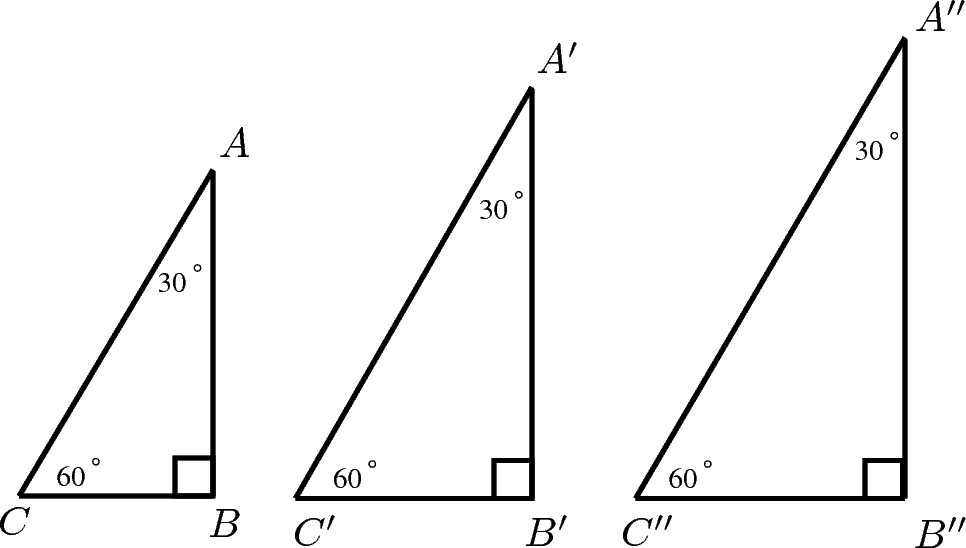
\includegraphics{col11306.imgs/m39405_MG10C15_002.png} % m39405;MG10C15\_002.png;;;6.0;8.5;
      \vspace{2pt}
    \vspace{.1in}
    \end{center}
 \end{figure}       
      \par 
    % \textbf{m39405*id78604}\par
          \begin{table}[H]
    % \begin{table}[H]
    % \\ '' '0'
        \begin{center}
      \label{m39405*id78604}
    \noindent
    \tabletail{%
        \hline
        \multicolumn{3}{|p{\mytableboxwidth}|}{\raggedleft \small \sl continued on next page}\\
        \hline
      }
      \tablelasttail{}
      \begin{xtabular}[t]{|l|l|l|}\hline
    % My position: 0
    % my spanname: 
    % my ct of spanspec: 0
    % my column-count: 3
    \multicolumn{3}{|c|}{Dividing lengths of sides (Ratios)}
     \tabularnewline\cline{1-1}\cline{2-2}\cline{3-3}
      %--------------------------------------------------------------------
                $\frac{AB}{BC}=\phantom{\rule{42.67912pt}{0ex}}$
               &
                $\frac{AB}{AC}=\phantom{\rule{42.67912pt}{0ex}}$
               &
                $\frac{CB}{AC}=\phantom{\rule{42.67912pt}{0ex}}$
              % make-rowspan-placeholders
     \tabularnewline\cline{1-1}\cline{2-2}\cline{3-3}
      %--------------------------------------------------------------------
                $\frac{{A}^{\text{'}}{B}^{\text{'}}}{{B}^{\text{'}}{C}^{\text{'}}}=\phantom{\rule{42.67912pt}{0ex}}$
               &
                $\frac{{A}^{\text{'}}{B}^{\text{'}}}{{A}^{\text{'}}{C}^{\text{'}}}=\phantom{\rule{42.67912pt}{0ex}}$
               &
                $\frac{{C}^{\text{'}}{B}^{\text{'}}}{{A}^{\text{'}}{C}^{\text{'}}}=\phantom{\rule{42.67912pt}{0ex}}$
              % make-rowspan-placeholders
     \tabularnewline\cline{1-1}\cline{2-2}\cline{3-3}
      %--------------------------------------------------------------------
                $\frac{{A}^{\text{'}\text{'}}{B}^{\text{'}\text{'}}}{{B}^{\text{'}\text{'}}{C}^{\text{'}\text{'}}}=\phantom{\rule{42.67912pt}{0ex}}$
               &
                $\frac{{A}^{\text{'}\text{'}}{B}^{\text{'}\text{'}}}{{A}^{\text{'}\text{'}}{C}^{\text{'}\text{'}}}=\phantom{\rule{42.67912pt}{0ex}}$
               &
                $\frac{{C}^{\text{'}\text{'}}{B}^{\text{'}\text{'}}}{{A}^{\text{'}\text{'}}{C}^{\text{'}\text{'}}}=\phantom{\rule{42.67912pt}{0ex}}$
              % make-rowspan-placeholders
     \tabularnewline\cline{1-1}\cline{2-2}\cline{3-3}
      %--------------------------------------------------------------------
    \end{xtabular}
      \end{center}
    \begin{center}{\small\bfseries Table 14.1}\end{center}
    \begin{caption}{\small\bfseries Table 14.1}\end{caption}
\end{table}
    \par
      \label{m39405*id79075}What observations can you make about the ratios of the sides?\par 
      \label{m39405*id79081}These equal ratios are used to define the trigonometric functions.\par 
      \label{m39405*id79087}\uline{Note:} In algebra, we often use the letter $x$ for our unknown variable (although we can use any other letter too, such as $a$, $b$, $k$, etc). In trigonometry, we often use the Greek symbol $\theta $ for an unknown angle (we also use $\alpha $ , $\beta $ , $\gamma $ etc). \par 
  \label{m39405**end}
%          \section{ The trig functions and 2-D problems}
%     \nopagebreak
%             \label{m39408} $ \hspace{-5pt}\begin{array}{cccccccccccc}   
\includegraphics[width=0.75cm]{col11306.imgs/summary_fullmarks.png} &   
\includegraphics[width=0.75cm]{col11306.imgs/summary_video.png} &   \end{array} $ \hspace{2 pt}\raisebox{-5 pt}{} {(section shortcode: MG10101 )} \par 
%     
%     
%     
    \label{m39408*cid5}
            \section{ Definition of the Trigonometric Functions}
            \nopagebreak
      \label{m39408*id79356}We are familiar with a function of the form $f\left(x\right)$ where $f$ is the function and $x$ is the argument. Examples are:\par 
      \label{m39408*id79391}\nopagebreak\noindent{}
    \begin{equation}
    \begin{array}{cccc}\hfill f\left(x\right)& =& {2}^{x}\hfill & \mathrm{\left(exponential\; function\right)}\hfill \\ \hfill g\left(x\right)& =& x+2\hfill & \mathrm{\left(linear\; function\right)}\hfill \\ \hfill h\left(x\right)& =& 2{x}^{2}\hfill & \mathrm{\left(parabolic\; function\right)}\hfill \end{array}\tag{14.4}
      \end{equation}
      \label{m39408*id79540}The basis of trigonometry are the \textsl{trigonometric functions}. There are three basic trigonometric functions:\par 
      \label{m39408*id79552}\begin{enumerate}[noitemsep, label=\textbf{\arabic*}. ] 
            \label{m39408*uid15}\item sine
\label{m39408*uid16}\item cosine
\label{m39408*uid17}\item tangent
\end{enumerate}
      \label{m39408*id79593}These are abbreviated to:\par 
      \label{m39408*id79596}\begin{enumerate}[noitemsep, label=\textbf{\arabic*}. ] 
            \label{m39408*uid18}\item sin
\label{m39408*uid19}\item cos
\label{m39408*uid20}\item tan
\end{enumerate}
      \label{m39408*id79636}These functions can be defined from a \textbf{right-angled triangle}, a triangle where one internal angle is 90 ${}^{\circ }$.\par 
      \label{m39408*id79660}Consider a right-angled triangle.\par 
      \label{m39408*id79664}
    \setcounter{subfigure}{0}
	\begin{figure}[H] % horizontal\label{m39408*id79667}
    \begin{center}
    \label{m39408*id79667!!!underscore!!!media}\label{m39408*id79667!!!underscore!!!printimage}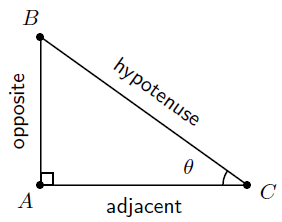
\includegraphics[width=200px]{col11306.imgs/m39408_MG10C15_003.png} % m39408;MG10C15\_003.png;;;6.0;8.5;
      \vspace{2pt}
    \vspace{.1in}
    \end{center}
 \end{figure}       
      \par 
      \label{m39408*id79673}In the right-angled triangle, we refer to the lengths of the three sides according to how they are placed in relation to the angle $\theta $. The side opposite to the right angle is labeled the \textsl{hypotenuse}, the side opposite $\theta $ is labeled \textsl{opposite}, the side next to $\theta $ is labeled \textsl{adjacent}. Note that the choice of non-90 degree internal angle is arbitrary. You can choose either internal angle and then define the adjacent and opposite sides accordingly. However, the hypotenuse remains the same regardless of which internal angle you are referring to (because it is ALWAYS opposite the right angle and ALWAYS the longest side).\par 
      \label{m39408*id79725}We define the trigonometric functions, also known as trigonometric identities, as:
\par 
      \label{m39408*uid21}\nopagebreak\noindent{}
    \begin{equation}
    \begin{array}{ccc}\hfill sin\theta & =& \frac{\mathrm{opposite}}{\mathrm{hypotenuse}}\hfill \\ \hfill cos\theta & =& \frac{\mathrm{adjacent}}{\mathrm{hypotenuse}}\hfill \\ \hfill tan\theta & =& \frac{\mathrm{opposite}}{\mathrm{adjacent}}\hfill \end{array}\tag{14.5}
      \end{equation}
      \label{m39408*id79934}These functions relate the lengths of the sides of a right-angled triangle to its interior angles.\par 
      \label{m39408*eip-55}
\begin{tabular}{cc}
	\hspace*{-50pt}\raisebox{-8 mm}{\hspace{-0.2in}
\includegraphics[width=0.75in]{col11306.imgs/psfact2.png} } & 
	\begin{minipage}{0.85\textwidth}
	\begin{note}
      {note: }The trig ratios are independent of the lengths of the sides of a triangle and depend only on the angles, this is why we can consider them to be functions of the angles.
	\end{note}
	\end{minipage}
	\end{tabular}
	\par
      \label{m39408*id79941}One way of remembering the definitions is to use the following mnemonic that is perhaps easier to remember:\par 
      \label{m39408*id79945}
    % \textbf{m39408*id79953}\par
          \begin{table}[H]
    % \begin{table}[H]
    % \\ '' '0'
        \begin{center}
      \label{m39408*id79953}
    \noindent
    \tabletail{%
        \hline
        \multicolumn{2}{|p{\mytableboxwidth}|}{\raggedleft \small \sl continued on next page}\\
        \hline
      }
      \tablelasttail{}
      \begin{xtabular}[t]{|l|l|}\hline
        \textbf{S}illy \textbf{O}ld \textbf{H}ens &
                  $\mathbf{S}\mathrm{in}=\frac{\mathbf{O}\mathrm{pposite}}{\mathbf{H}\mathrm{ypotenuse}}$
                % make-rowspan-placeholders
     \tabularnewline\cline{1-1}\cline{2-2}
      %--------------------------------------------------------------------
        \textbf{C}ackle \textbf{A}nd \textbf{H}owl &
                  $\mathbf{C}\mathrm{os}=\frac{\mathbf{A}\mathrm{djacent}}{\mathbf{H}\mathrm{ypotenuse}}$
                % make-rowspan-placeholders
     \tabularnewline\cline{1-1}\cline{2-2}
      %--------------------------------------------------------------------
        \textbf{T}ill \textbf{O}ld \textbf{A}ge &
                  $\mathbf{T}\mathrm{an}=\frac{\mathbf{O}\mathrm{pposite}}{\mathbf{A}\mathrm{djacent}}$
                % make-rowspan-placeholders
     \tabularnewline\cline{1-1}\cline{2-2}
      %--------------------------------------------------------------------
    \end{xtabular}
      \end{center}
    \begin{center}{\small\bfseries Table 14.2}\end{center}
    \begin{caption}{\small\bfseries Table 14.2}\end{caption}
\end{table}
    \par
      \par 
\label{m39408*eip-186}You may also hear people saying Soh Cah Toa. This is just another way to remember the trig functions.\par \label{m39408*notfhsst!!!underscore!!!id934}
\begin{tabular}{cc}
	   \hspace*{-50pt}\raisebox{-8 mm}{ 
\includegraphics[width=0.5in]{col11306.imgs/pstip2.png}  }& 
	\begin{minipage}{0.85\textwidth}
	\begin{note}
      {tip: }The definitions of opposite, adjacent and hypotenuse are only applicable when you are working with right-angled triangles! Always check to make sure your triangle has a right-angle before you use them, otherwise you will get the wrong answer. We will find ways of using our knowledge of right-angled triangles to deal with the trigonometry of non right-angled triangles in Grade 11.
	\end{note}
	\end{minipage}
	\end{tabular}
	\par
\label{m39408*secfhsst!!!underscore!!!id935}
            \subsection{  Exercises : Definitions of Trigonometric Functions }
            \nopagebreak
      \label{m39408*id80155}\begin{enumerate}[noitemsep, label=\textbf{\arabic*}. ] 
            \label{m39408*uid22}\item In each of the following triangles, state whether $a$, $b$ and $c$ are the hypotenuse, opposite or adjacent sides of the triangle with respect to the marked angle.
    \setcounter{subfigure}{0}
	\begin{figure}[H] % horizontal\label{m39408*id80200}
    \begin{center}
    \label{m39408*id80200!!!underscore!!!media}\label{m39408*id80200!!!underscore!!!printimage}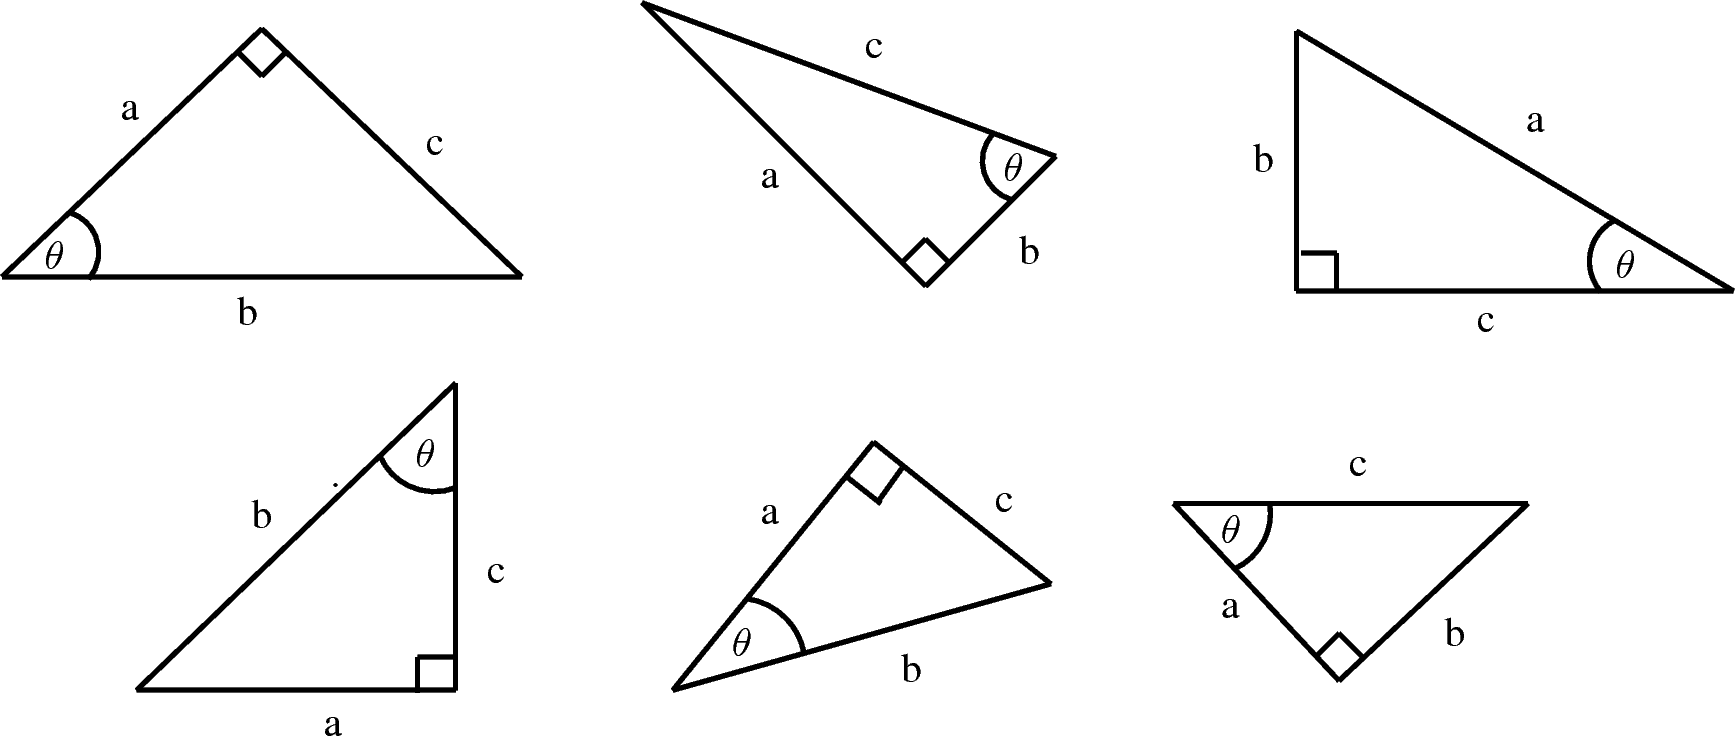
\includegraphics{col11306.imgs/m39408_MG10C15_004.png} % m39408;MG10C15\_004.png;;;6.0;8.5;
      \vspace{2pt}
    \vspace{.1in}
    \end{center}
 \end{figure}       \label{m39408*uid23}\item Complete each of the following, the first has been done for you
    \setcounter{subfigure}{0}
	\begin{figure}[H] % horizontal\label{m39408*id80226}
    \begin{center}
    \label{m39408*id80226!!!underscore!!!media}\label{m39408*id80226!!!underscore!!!printimage}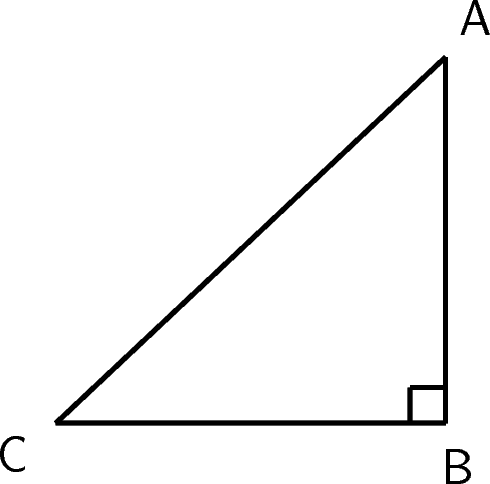
\includegraphics{col11306.imgs/m39408_MG10C15_005.png} % m39408;MG10C15\_005.png;;;6.0;8.5;
      \vspace{2pt}
    \vspace{.1in}
    \end{center}
 \end{figure}       \label{m39408*id80237}\nopagebreak\noindent{}
    \begin{equation}
    \begin{array}{ccc}\hfill a\right)sin\hat{A}& =& \frac{\mathrm{opposite}}{\mathrm{hypotenuse}}=\frac{CB}{AC}\hfill \\ \hfill b\right)cos\hat{A}& =& \\ \hfill c\right)tan\hat{A}& =\end{array}\tag{14.6}
      \end{equation}
    \label{m39408*id80376}\nopagebreak\noindent{}
    \begin{equation}
    \begin{array}{ccc}& d\right)& sin\hat{C}=\hfill \\ & e\right)& cos\hat{C}=\hfill \\ & f\right)& tan\hat{C}=\hfill \end{array}\tag{14.7}
      \end{equation}
    \label{m39408*uid24}\item Complete each of the following without a calculator:
    \setcounter{subfigure}{0}
	\begin{figure}[H] % horizontal\label{m39408*id80508}
    \begin{center}
    \label{m39408*id80508!!!underscore!!!media}\label{m39408*id80508!!!underscore!!!printimage}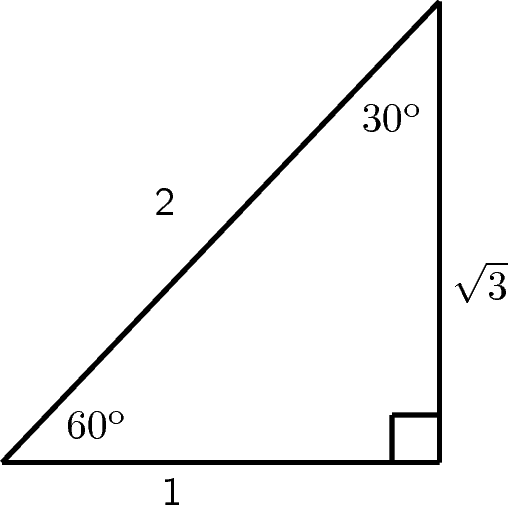
\includegraphics{col11306.imgs/m39408_MG10C15_006.png} % m39408;MG10C15\_006.png;;;6.0;8.5;
      \vspace{2pt}
    \vspace{.1in}
    \end{center}
 \end{figure}       \label{m39408*id80519}\nopagebreak\noindent{}
    \begin{equation}
    \begin{array}{ccc}\hfill sin60& =& \\ \hfill cos30& =& \\ \hfill tan60& =\end{array}\tag{14.8}
      \end{equation}
    \setcounter{subfigure}{0}
	\begin{figure}[H] % horizontal\label{m39408*id80587}
    \begin{center}
    \label{m39408*id80587!!!underscore!!!media}\label{m39408*id80587!!!underscore!!!printimage}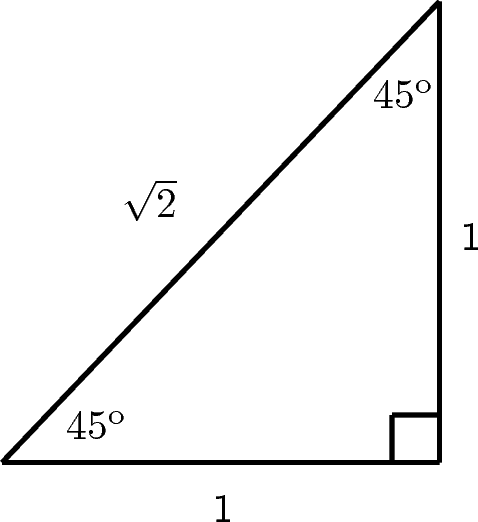
\includegraphics{col11306.imgs/m39408_MG10C15_007.png} % m39408;MG10C15\_007.png;;;6.0;8.5;
      \vspace{2pt}
    \vspace{.1in}
    \end{center}
 \end{figure}       \label{m39408*id80598}\nopagebreak\noindent{}
    \begin{equation}
    \begin{array}{ccc}\hfill sin45& =& \\ \hfill cos45& =& \\ \hfill tan45& =\end{array}\tag{14.9}
      \end{equation}
    \end{enumerate}
      \label{m39408*id80673}For most angles $\theta $, it is very difficult to calculate the values of $sin\theta $, $cos\theta $ and $tan\theta $. One usually needs to use a calculator to do so. However, we saw in the above Activity that we could work these values out for some special angles. Some of these angles are listed in the table below, along with the values of the trigonometric functions at these angles. Remember that the lengths of the sides of a right angled triangle must obey Pythagoras' theorem. The square of the hypotenuse (side opposite the 90 degree angle) equals the sum of the squares of the two other sides.\par 
    % \textbf{m39408*id80733}\par
          \begin{table}[H]
    % \begin{table}[H]
    % \\ '' '0'
        \begin{center}
      \label{m39408*id80733}
    \noindent
    \tabletail{%
        \hline
        \multicolumn{7}{|p{\mytableboxwidth}|}{\raggedleft \small \sl continued on next page}\\
        \hline
      }
      \tablelasttail{}
      \begin{xtabular}[t]{|l|l|l|l|l|l|l|}\hline
         &
                ${0}^{\circ }$
               &
                ${30}^{\circ }$
               &
                ${45}^{\circ }$
               &
                ${60}^{\circ }$
               &
                ${90}^{\circ }$
               &
                ${180}^{\circ }$
              % make-rowspan-placeholders
     \tabularnewline\cline{1-1}\cline{2-2}\cline{3-3}\cline{4-4}\cline{5-5}\cline{6-6}\cline{7-7}
      %--------------------------------------------------------------------
                $cos\theta $
               &
        1 &
                $\frac{\sqrt{3}}{2}$
               &
                $\frac{1}{\sqrt{2}}$
               &
                $\frac{1}{2}$
               &
        0 &
                $-1$
              % make-rowspan-placeholders
     \tabularnewline\cline{1-1}\cline{2-2}\cline{3-3}\cline{4-4}\cline{5-5}\cline{6-6}\cline{7-7}
      %--------------------------------------------------------------------
                $sin\theta $
               &
        0 &
                $\frac{1}{2}$
               &
                $\frac{1}{\sqrt{2}}$
               &
                $\frac{\sqrt{3}}{2}$
               &
        1 &
        0% make-rowspan-placeholders
     \tabularnewline\cline{1-1}\cline{2-2}\cline{3-3}\cline{4-4}\cline{5-5}\cline{6-6}\cline{7-7}
      %--------------------------------------------------------------------
                $tan\theta $
               &
        0 &
                $\frac{1}{\sqrt{3}}$
               &
        1 &
                $\sqrt{3}$
               &
                $-$
               &
        0% make-rowspan-placeholders
     \tabularnewline\cline{1-1}\cline{2-2}\cline{3-3}\cline{4-4}\cline{5-5}\cline{6-6}\cline{7-7}
      %--------------------------------------------------------------------
    \end{xtabular}
      \end{center}
    \begin{center}{\small\bfseries Table 14.3}\end{center}
    \begin{caption}{\small\bfseries Table 14.3}\end{caption}
\end{table}
    \par
      \label{m39408*id81112}These values are useful when asked to solve a problem involving trig functions \textsl{without} using a calculator.\par 
\section{Reciprocal Functions}
\label{m39408*eip-466}Each of the trigonometric functions has a reciprocal that has a special name. The three reciprocals are cosecant (or cosec), secant (or sec) and cotangent (or cot). These reciprocals are given below:
\label{m39408*eid64932}\nopagebreak\noindent{}
    \begin{equation}
    \begin{array}{ccc}cosec\theta & =& \frac{1}{sin\theta }\\ sec\theta & =& \frac{1}{cos\theta }\\ cot\theta & =& \frac{1}{tan\theta }\end{array}\tag{14.10}
      \end{equation}
\par \label{m39408*eip-520}We can also define these reciprocals for any right angled triangle:
\label{m39408*eid96732}\nopagebreak\noindent{}

    \begin{equation}
    \begin{array}{ccc}\hfill cosec\theta & =& \frac{\mathrm{hypotenuse}}{\mathrm{opposite}}\hfill \\ \hfill sec\theta & =& \frac{\mathrm{hypotenuse}}{\mathrm{adjacent}}\hfill \\ \hfill cot\theta & =& \frac{\mathrm{adjacent}}{\mathrm{opposite}}\hfill \end{array}\tag{14.11}
      \end{equation}
\par \par
            \label{m39408*secfhsst!!!underscore!!!id1130}\vspace{.5cm} 
      \noindent
      \hspace*{-30pt}
\includegraphics[width=0.5in]{col11306.imgs/pspencil2.png}   \raisebox{25mm}{   
      \begin{mdframed}[linewidth=4, leftmargin=40, rightmargin=40]  
      \begin{exercise}
    \noindent\textbf{Exercise 14.1:  Finding Lengths }
      \label{m39408*probfhsst!!!underscore!!!id1131}
      \label{m39408*id81134}Find the length of x in the following triangle.\par 
      \label{m39408*id81140}
    \setcounter{subfigure}{0}
	\begin{figure}[H] % horizontal\label{m39408*id81141}
    \begin{center}
    \label{m39408*id81141!!!underscore!!!media}\label{m39408*id81141!!!underscore!!!printimage}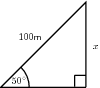
\includegraphics[width=150px]{col11306.imgs/m39408_MG10C15_008.png} % m39408;MG10C15\_008.png;;;6.0;8.5;
      \vspace{2pt}
    \vspace{.1in}
    \end{center}
 \end{figure}       
      \par 
      \vspace{5pt}
      \label{m39408*solfhsst!!!underscore!!!id1143}\noindent\textbf{Solution to Exercise } \label{m39408*listfhsst!!!underscore!!!id1143}\begin{enumerate}[noitemsep, label=\textbf{Step} \textbf{\arabic*}. ] 
            \leftskip=20pt\rightskip=\leftskip\item  
      \label{m39408*id81169}In this case you have an angle (${50}^{\circ }$), the opposite side and the hypotenuse.\par 
      \label{m39408*id81188}So you should use $sin$\par 
      \label{m39408*id81204}\nopagebreak\noindent{}
        
    \begin{equation}
    sin{50}^{\circ }=\frac{x}{100}\tag{14.12}
      \end{equation}
      \item  
      \label{m39408*id81247}\nopagebreak\noindent{}
        
    \begin{equation}
    \ensuremath{\Rightarrow}x=100\ensuremath{\times}sin{50}^{\circ }\tag{14.13}
      \end{equation}
      \item  
      \label{m39408*id81284}Use the sin
 button on your calculator\par 
      \label{m39408*id81293}\nopagebreak\noindent{}
        
    \begin{equation}
    \ensuremath{\Rightarrow}x=76.6\mathrm{m}\tag{14.14}
      \end{equation}
      \end{enumerate}
    \end{exercise}
    \end{mdframed}
    }
    \noindent
\par
    \noindent
\label{m39408*eip-200}In the previous example we used ${\mathrm{tan}}^{-1}$. This is simply the inverse of the tan function. Sin and cos also have inverses. All this means is that we want to find the angle that makes the expression true and so we must move the tan (or sin or cos) to the other side of the equals sign and leave the angle where it is. Sometimes the reciprocal trigonometric functions are also referred to as the 'inverse trigonometric functions'. You should note, however that ${\mathrm{tan}}^{-1}$ and $\mathrm{cot}$ are definitely NOT the same thing. \par \label{m39408*eip-358}The following videos provide a summary of what you have learnt so far.
    \setcounter{subfigure}{0}
	\begin{figure}[H] % horizontal\label{m39408*trigonometry-1}
    \textnormal{Trigonometry - 1}\vspace{.1in} \nopagebreak
  \label{m39408*yt-media}\label{m39408*yt-video}
            \raisebox{-5 pt}{ 
\includegraphics[width=0.5cm]{col11306.imgs/summary_www.png}} { (Video:  MG10102 )}
      \vspace{2pt}
    \vspace{.1in}
 \end{figure}       \par \label{m39408*eip-33}
    \setcounter{subfigure}{0}
	\begin{figure}[H] % horizontal\label{m39408*trigonometry-2}
    \textnormal{Khan academy video on trigonometry - 2}\vspace{.1in} \nopagebreak
  \label{m39408*yt-media2}\label{m39408*yt-video2}
            \raisebox{-5 pt}{ 
\includegraphics[width=0.5cm]{col11306.imgs/summary_www.png}} { (Video:  MG10103 )}
      \vspace{2pt}
    \vspace{.1in}
 \end{figure}       \par \label{m39408*secfhsst!!!underscore!!!id1260}
            \subsection{Exercise: Finding Lengths }
            \nopagebreak
            \label{m39408*id81582}Find the length of the sides marked with letters. Give answers correct to 2 decimal places.
    \setcounter{subfigure}{0}
	\begin{figure}[H] % horizontal\label{m39408*id81592}
    \begin{center}
    \label{m39408*id81592!!!underscore!!!media}\label{m39408*id81592!!!underscore!!!printimage}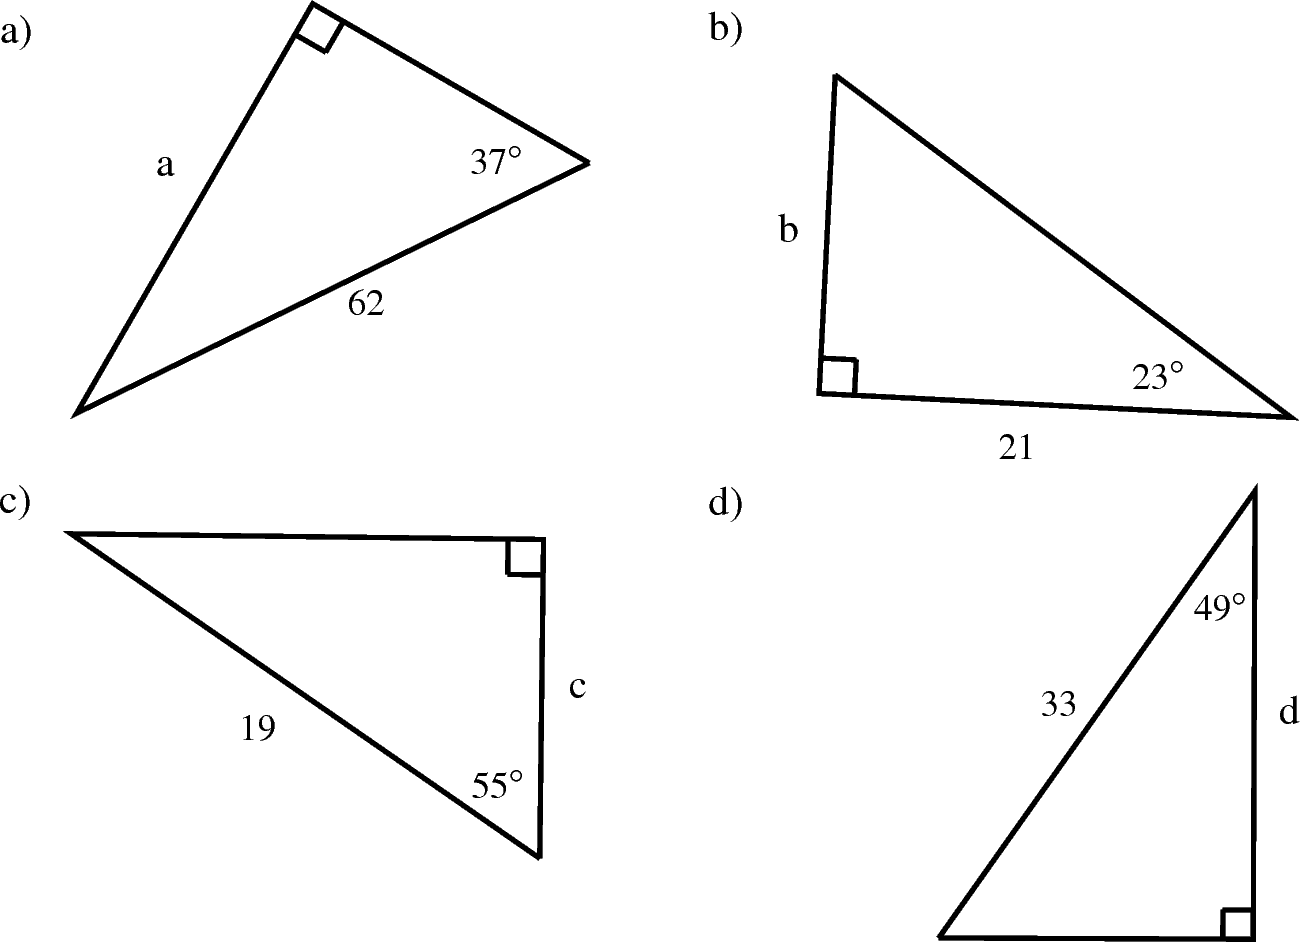
\includegraphics{col11306.imgs/m39408_MG10C15_010.png} % m39408;MG10C15\_010.png;;;6.0;8.5;
      \vspace{2pt}
    \vspace{.1in}
    \end{center}
 \end{figure}       
    \setcounter{subfigure}{0}
	\begin{figure}[H] % horizontal\label{m39408*id816001}
    \begin{center}
    \label{m39408*id816001!!!underscore!!!media}\label{m39408*id816001!!!underscore!!!printimage}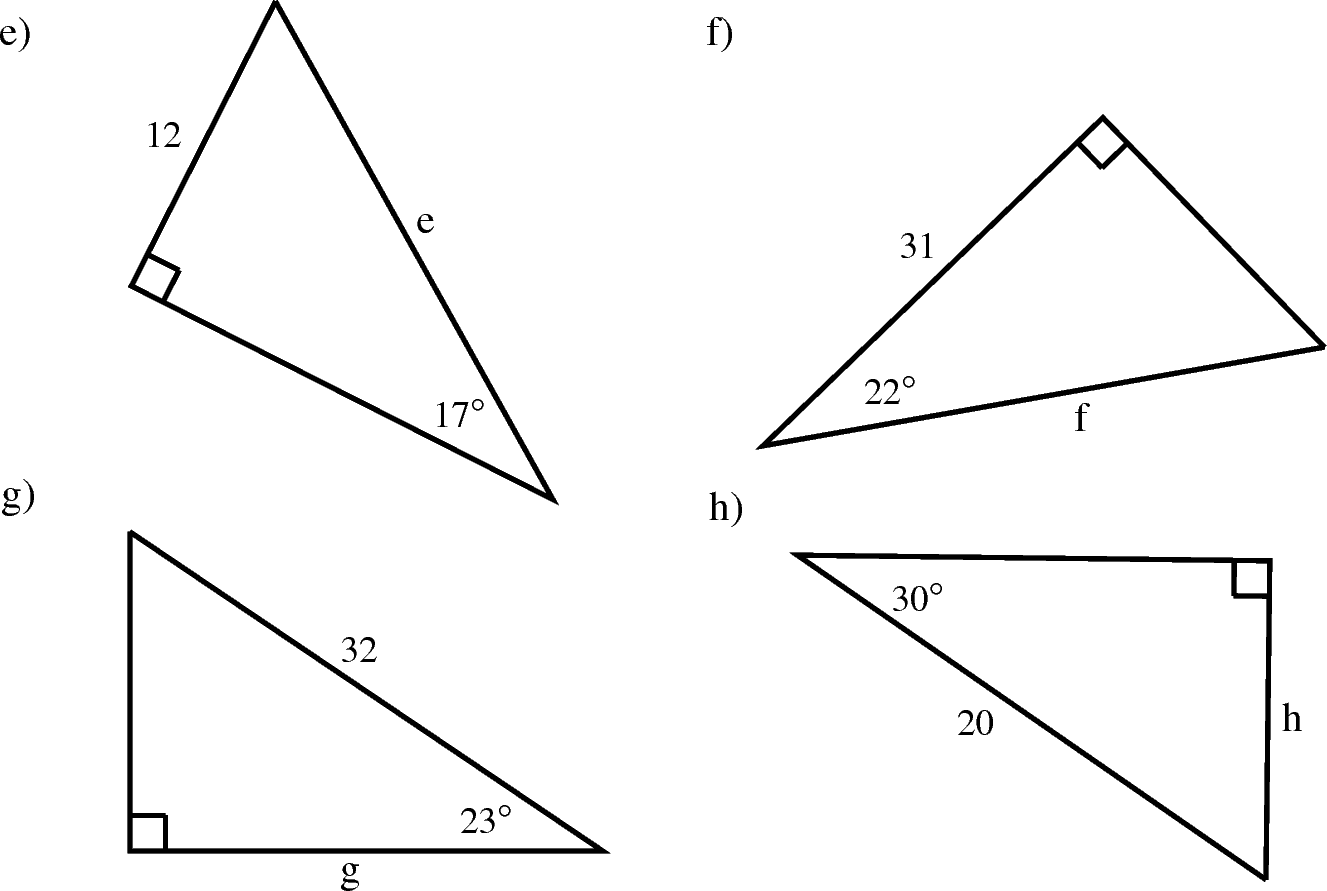
\includegraphics{col11306.imgs/m39408_MG10C15_011.png} % m39408;MG10C15\_011.png;;;6.0;8.5;
      \vspace{2pt}
    \vspace{.1in}
    \end{center}
 \end{figure}       
              \par 
    \label{m39408*eip-403}
\par \raisebox{-5 pt}{
\includegraphics[width=0.5cm]{col11306.imgs/summary_www.png}} Find the answers with the shortcodes:
 \par \begin{tabular}[h]{cccccc}
 (1.) lc1  & \end{tabular}
\section{Finding an Angle}
  \label{m39408*secfhsst!!!underscore!!!id1199}\vspace{.5cm} 
      \noindent
      \hspace*{-30pt}
\includegraphics[width=0.5in]{col11306.imgs/pspencil2.png}   \raisebox{25mm}{   
      \begin{mdframed}[linewidth=4, leftmargin=40, rightmargin=40]  
      \begin{exercise}
    \noindent\textbf{Exercise 14.2:  Finding Angles }
      \label{m39408*probfhsst!!!underscore!!!id1200}
      \label{m39408*id81349}Find the value of $\theta $ in the following triangle.\par 
      \label{m39408*id81364}
    \setcounter{subfigure}{0}
	\begin{figure}[H] % horizontal\label{m39408*id81368}
    \begin{center}
    \label{m39408*id81368!!!underscore!!!media}\label{m39408*id81368!!!underscore!!!printimage}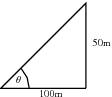
\includegraphics[width=150px]{col11306.imgs/m39408_MG10C15_009.png} % m39408;MG10C15\_009.png;;;6.0;8.5;
      \vspace{2pt}
    \vspace{.1in}
    \end{center}
 \end{figure}       
 \par 
      \vspace{5pt}
      \label{m39408*solfhsst!!!underscore!!!id1206}\noindent\textbf{Solution to Exercise } \label{m39408*listfhsst!!!underscore!!!id1206}\begin{enumerate}[noitemsep, label=\textbf{Step} \textbf{\arabic*}. ] 
            \leftskip=20pt\rightskip=\leftskip\item  
      \label{m39408*id81396}In this case you have the opposite side and the hypotenuse to the angle $\theta $.\par 
      \label{m39408*id81410}So you should use $tan$\par 
      \label{m39408*id81425}\nopagebreak\noindent{}
        
    \begin{equation}
    tan\theta =\frac{50}{100}\tag{14.15}
      \end{equation}
      \item  
      \label{m39408*id81454}\nopagebreak\noindent{}
    \begin{equation}
    tan\theta =0.5\tag{14.16}
      \end{equation}
      \item  
      \label{m39408*id81485}Since you are finding the \textsl{angle},\par 
      \label{m39408*id81494}use ${tan}^{-1}$
 on your calculator\par 
      \label{m39408*id81524}Don't forget to set your calculator to `deg' mode!\par 
      \label{m39408*id81529}\nopagebreak\noindent{}
    \begin{equation}
    \theta =26.{6}^{\circ }\tag{14.17}
      \end{equation}
      \end{enumerate}
    \end{exercise}
    \end{mdframed}
    }
% \section{Special Angles}
\section{Defining Ratios in the Cartesian Plane}
\label{m39411*eip-945}
%             \subsection{ The trig functions for any angle}
            \nopagebreak
            \label{m39411*eip-156}So far we have defined the trig functions using right angled triangles. We can now extend these definitions to any angle. We do this by noting that the definitions do not rely on the lengths of the sides of the triangle, but only on the angle. So if we plot any point on the Cartesian plane and then draw a line from the origin to that point, we can work out the angle of that line. In Figure~14.15 points P and Q have been plotted. A line from the origin to each point is drawn. The dotted lines show how we can construct right angle triangles for each point. Now we can find the angles A and B.
\par \label{m39411*eip-970}
    \setcounter{subfigure}{0}
	\begin{figure}[H] % horizontal\label{m39411*id63458}
    \begin{center}
    \label{m39411*id63458!!!underscore!!!media}\label{m39411*id63458!!!underscore!!!printimage}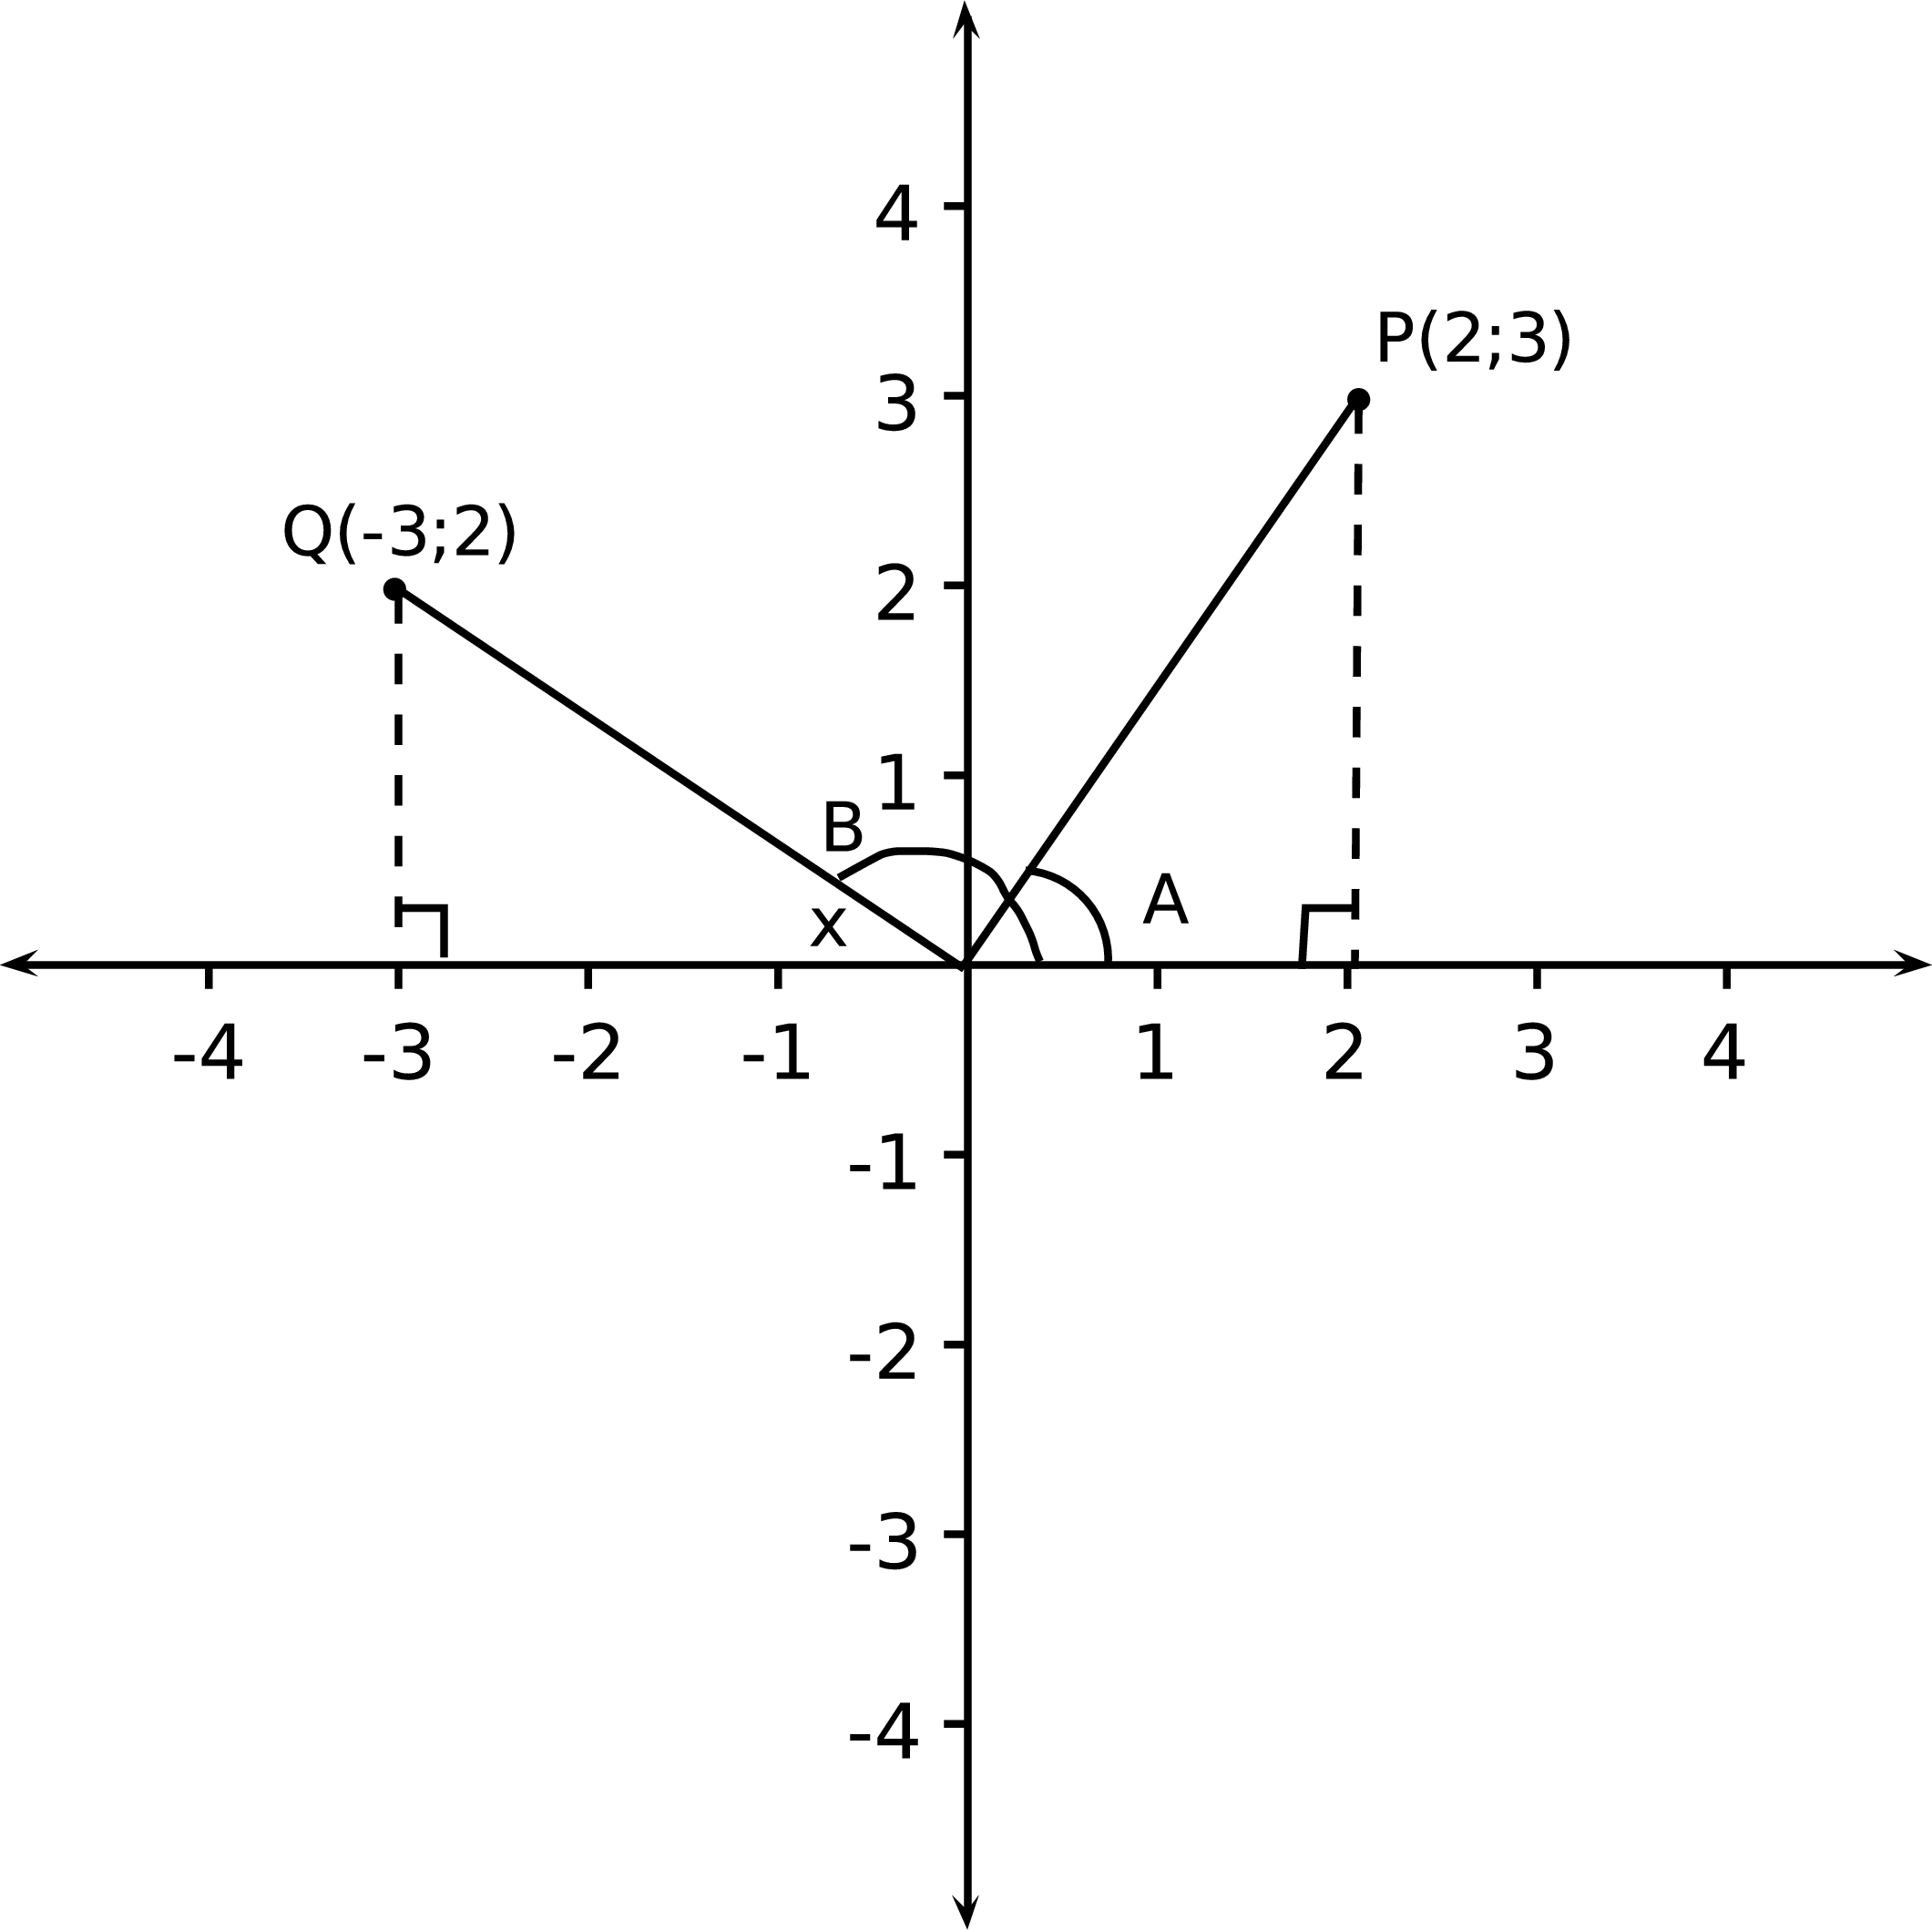
\includegraphics[width=300px]{col11306.imgs/m39411_trigfunc1.png} % m39411;trigfunc1.png;;;6.0;8.5;
      \vspace{2pt}
    \vspace{.1in}
    \end{center}
 \end{figure}       \par \label{m39411*eip-9}You should find the angle A is $63,{43}^{\circ }$. For angle B, you first work out x ($33,{69}^{\circ }$) and then B is ${180}^{\circ }-33,{69}^{\circ }=146,{31}^{\circ }$. But what if we wanted to do this without working out these angles and figuring out whether to add or subtract 180 or 90? Can we use the trig functions to do this? Consider point P in Figure~14.15. To find the angle you would have used one of the trig functions, e.g. $\mathrm{tan}\phantom{\rule{1pt}{0ex}}\theta $. You should also have noted that the side adjacent to the angle was just the x-co-ordinate and that the side opposite the angle was just the y-co-ordinate. But what about the hypotenuse? Well, you can find that using Pythagoras since you have two sides of a right angled triangle. If we were to draw a circle centered on the origin, then the length from the origin to point P is the radius of the circle, which we denote r. Now we can rewrite all our trig functions in terms of x, y and r. But how does this help us to find angle B? Well, we know that from point Q to the origin is r, and we have the co-ordinates of Q. So we simply use the newly defined trig functions to find angle B! (Try it for yourself and confirm that you get the same answer as before.) One final point to note is that when we go anti-clockwise around the Cartesian plane the angles are positive and when we go clockwise around the Cartesian plane, the angles are negative. \par \label{m39411*eip-634}So we get the following definitions for the trig functions:
\par \label{m39411*eip-169}\nopagebreak\noindent{}
    \begin{equation}
    \begin{array}{ccc}\hfill sin\theta & =& \frac{x}{r}\hfill \\ \hfill cos\theta & =& \frac{y}{r}\hfill \\ \hfill tan\theta & =& \frac{y}{x}\hfill \end{array}\tag{14.20}
      \end{equation}
    \label{m39411*eip-102}But what if the x- or y-co-ordinate is negative? Do we ignore that, or is there some way to take that into account? The answer is that we do not ignore it. The sign in front of the x- or y-co-ordinate tells us whether or not sin, cos and tan are positive or negative. We divide the Cartesian plane into quadrants and then we can use Figure~14.16 to tell us whether the trig function is positive or negative. This diagram is known as the CAST diagram.\par \label{m39411*eip-216}
    \setcounter{subfigure}{0}
\section{CAST Diagram}
\begin{figure}[H] % horizontal\label{m39411*id63358}
    \begin{center}
    \label{m39411*id63358!!!underscore!!!media}\label{m39411*id63358!!!underscore!!!printimage}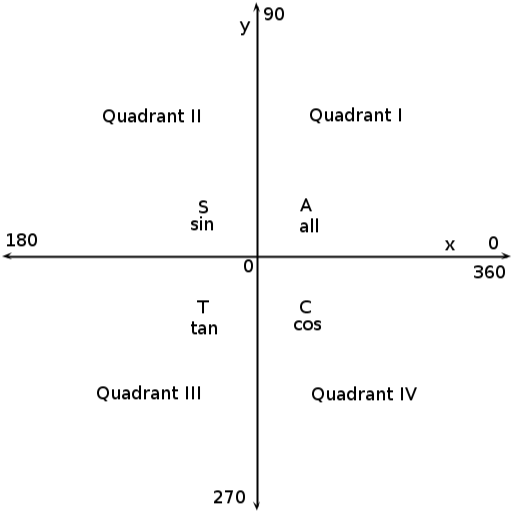
\includegraphics[width=300px]{col11306.imgs/m39411_CAST.png} % m39411;CAST.png;;;6.0;8.5;
      \vspace{2pt}
    \vspace{.1in}
    \end{center}
 \end{figure}       \par \label{m39411*eip-927}We can also extend the definitions of the reciprocals in the same way:
\label{m39411*id89342}\nopagebreak\noindent{}

    \begin{equation}
    \begin{array}{ccc}\hfill cosec\theta & =& \frac{r}{x}\hfill \\ \hfill sec\theta & =& \frac{r}{y}\hfill \\ \hfill cot\theta & =& \frac{x}{y}\hfill \end{array}\tag{14.21}
      \end{equation}
\par
 \par
            \label{m39411*eip-986}\vspace{.5cm} 
      \noindent
      \hspace*{-30pt}
\includegraphics[width=0.5in]{col11306.imgs/pspencil2.png}   \raisebox{25mm}{   
      \begin{mdframed}[linewidth=4, leftmargin=40, rightmargin=40]  
      \begin{exercise}
    \noindent\textbf{Exercise 14.4: Finding the angle}\label{m39411*probfhsst!!!underscore!!!id182}
        \label{m39411*id8189}Points R(-1;-3) and point S(3;-3) are plotted in the diagram below. Find the angles $\alpha $ and $\beta $. \par 
        \label{m39411*id8128}
    \setcounter{subfigure}{0}
	\begin{figure}[H] % horizontal\label{m39411*id8199}
    \begin{center}
    \label{m39411*id8199!!!underscore!!!media}\label{m39411*id8199!!!underscore!!!printimage}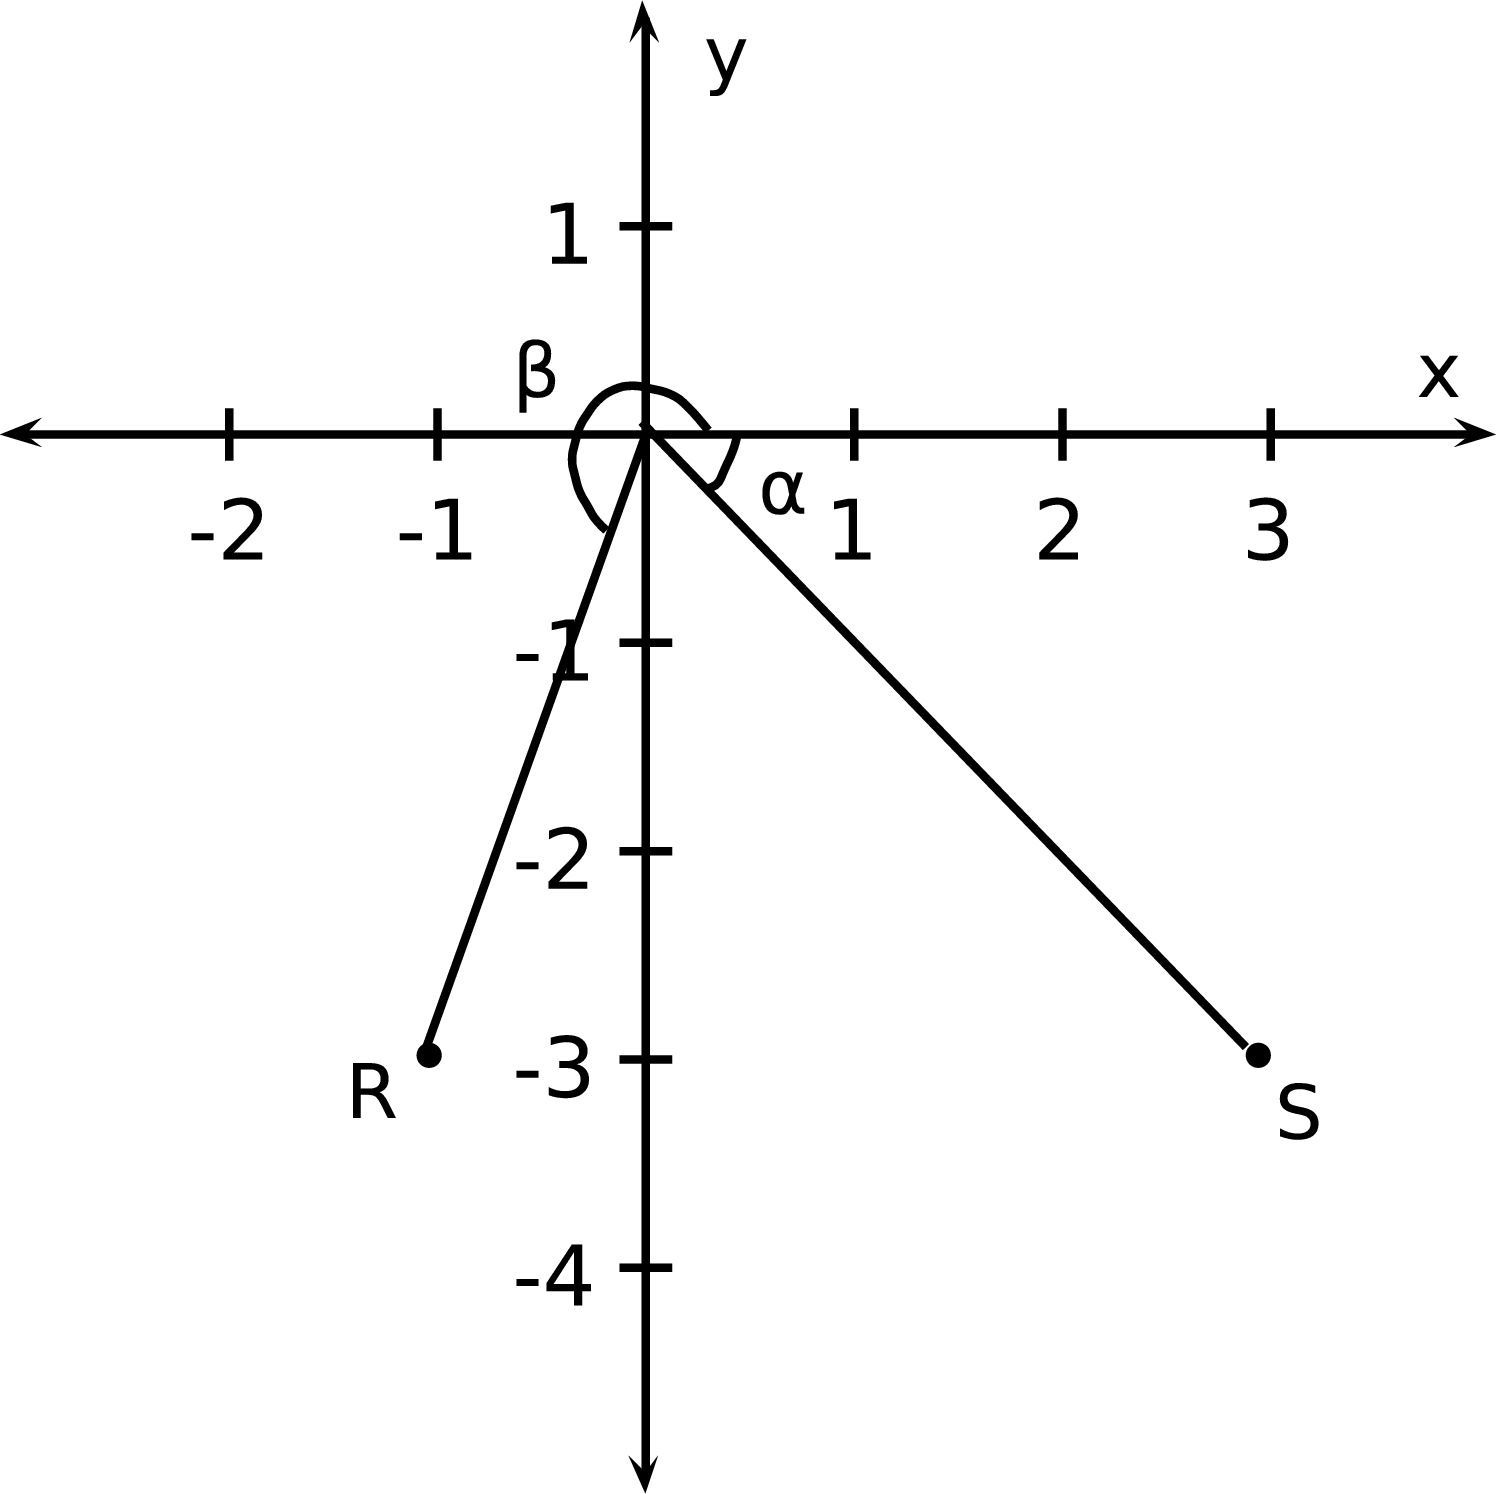
\includegraphics[width=300px]{col11306.imgs/m39411_qtrig.png} % m39411;qtrig.png;;;6.0;8.5;
      \vspace{2pt}
    \vspace{.1in}
    \end{center}
 \end{figure}       
        \par 
        \vspace{5pt}
        \label{m39411*solfhsst!!!underscore!!!id194}\noindent\textbf{Solution to Exercise } \label{m39411*listfhsst!!!underscore!!!id194}\begin{enumerate}[noitemsep, label=\textbf{Step} \textbf{\arabic*}. ] 
            \leftskip=20pt\rightskip=\leftskip\item  
        \label{m39411*id81936}We have the co-ordinates of the points R and S. We are required to find two angles. Angle $\beta $ is positive and angle $\alpha $ is negative.\par 
        \item  
        \label{m39411*id8267}We use tan to find $\beta $, since we are only given x and y. We note that we are in the third quadrant, where tan is positive.\par 
        \label{m39411*id82128}\nopagebreak\noindent{}
    \begin{equation}
    \begin{array}{ccc}\hfill tan\left(\beta \right)& =& \frac{y}{x}\hfill \\ \hfill tan\left(\beta \right)& =& \frac{-3}{-1}\hfill \\ \beta & =& {tan}^{-1}\left(3\right)\hfill \\ \beta & =& 71,{57}^{\circ }\hfill \end{array}\tag{14.22}
      \end{equation}
        \item  
\label{m39411*id9732}We use tan to calculate $\alpha $, since we are only given x and y. We also note that we are in the fourth quadrant, where tan is positive.
\par 
        \label{m39411*id8254}\nopagebreak\noindent{}
    \begin{equation}
    \begin{array}{ccc}\hfill tan\left(\alpha \right)& =& \frac{y}{x}\hfill \\ \hfill tan\left(\alpha \right)& =& \frac{-3}{3}\hfill \\ \alpha & =& {tan}^{-1}\left(-1\right)\hfill \\ \alpha & =& {-45}^{\circ }\hfill \end{array}\tag{14.23}
      \end{equation}
        \item  
        \label{m39411*id827} Angle $\alpha $ is ${-45}^{\circ }$ and angle $\beta $ is $71,{57}^{\circ }$
 \par 
        \end{enumerate}
    \end{exercise}
    \end{mdframed}
    }
    \noindent
  \label{m39411*eip-94}
\begin{tabular}{cc}
	\hspace*{-50pt}\raisebox{-8 mm}{\hspace{-0.2in}
\includegraphics[width=0.75in]{col11306.imgs/psfact2.png} } & 
	\begin{minipage}{0.85\textwidth}
	\begin{note}
      {note: }You should observe that in the worked example above, the angle $\alpha $ is simply the angle that line OS makes with the x-axis. So if you are asked to find out what angle a line makes with the x- or y-axes, then you can use trigonometry!
	\end{note}
	\end{minipage}
	\end{tabular}
	\par
      \label{m39411*eip-797}
\begin{tabular}{cc}
	\hspace*{-50pt}\raisebox{-8 mm}{\hspace{-0.2in}
\includegraphics[width=0.75in]{col11306.imgs/psfact2.png} } & 
	\begin{minipage}{0.85\textwidth}
	\begin{note}
      {note: }The CAST diagram can be generalized to a very powerful tool for solving trigonometric functions by hand (that is, without a calculator) called \textsl{the unit circle}. You may or may not touch on this in Grade 11 or 12.
	\end{note}
	\end{minipage}
	\end{tabular}
	\par
      \label{m39411*eip-822}
\section{Solving Trigonometric Equations}
%  \section{ Solving simple trigonometric equations}
            \nopagebreak
            \label{m39411*eip-361}
Using what we have learnt about trig functions we can now solve some simple trig equations. We use the principles from Equations and Inequalities\footnote{\raggedright{}"Equations and Inequalities - Grade 10 [CAPS]" <http://http://cnx.org/content/m38372/latest/>} to help us solve trig equations. 
\par \label{m39411*eip-301}
\begin{tabular}{cc}
	\hspace*{-50pt}\raisebox{-8 mm}{\hspace{-0.2in}
\includegraphics[width=0.75in]{col11306.imgs/psfact2.png} } & 
	\begin{minipage}{0.85\textwidth}
	\begin{note}
      {note: }It is important to note that in general $2sin\theta \ne sin\left(2\theta \right)$. In other words doubling (or multiplying by 2) has a different effect from doubling the angle.
	\end{note}
	\end{minipage}
	\end{tabular}
	\par
      \label{m39411*eip-618}\vspace{.5cm} 
      \noindent
      \hspace*{-30pt}
\includegraphics[width=0.5in]{col11306.imgs/pspencil2.png}   \raisebox{25mm}{   
      \begin{mdframed}[linewidth=4, leftmargin=40, rightmargin=40]  
      \begin{exercise}
    \noindent\textbf{Exercise 14.5}\label{m39411*eip-440}
  \label{m39411*eip-811}
   Solve the following trig equation: $3cos\left(2x+{38}^{\circ }\right)+3=2$
  \par 
\vspace{5pt}
\label{m39411*eip-616}\noindent\textbf{Solution to Exercise }
 \label{m39411*id987324}\begin{enumerate}[noitemsep, label=\textbf{Step} \textbf{\arabic*}. ] 
            \leftskip=20pt\rightskip=\leftskip\item 
\label{m39411*id0832}\nopagebreak\noindent{}
    \begin{equation}
    \begin{array}{ccc}\hfill 3cos\left(2x+{38}^{\circ }\right)& =& 2-3\hfill \\ \hfill cos\left(2x+{38}^{\circ }\right)& =& \frac{-1}{3}\hfill \\ \hfill \left(2x+{38}^{\circ }\right)& =& 107,{46}^{\circ }\hfill \\ \hfill 2x& =& 107,{46}^{\circ }-{38}^{\circ }\hfill \\ \hfill 2x& =& 69,{46}^{\circ }\hfill \\ \hfill x& =& 34,{73}^{\circ }\hfill \end{array}\tag{14.24}
      \end{equation}
\item 
$x=34,{73}^{\circ }$
\end{enumerate}
    \end{exercise}
    \end{mdframed}
    }
    \noindent
  \label{m39411*eip-858}
\begin{tabular}{cc}
	\hspace*{-50pt}
\includegraphics[width=0.5in]{col11306.imgs/psbulb2.png}  & 
	\begin{minipage}{0.85\textwidth}
	\begin{note}
      {aside: }In grade 11 and 12, you will learn more about solving trig equations. 
	\end{note}
	\end{minipage}
	\end{tabular}
\section{Applications}
 \label{m39411*id81626}Trigonometry was probably invented in ancient civilisations to solve practical problems such as building construction and navigating by the stars. In this section we will show how trigonometry can be used to solve some other practical problems.\par 
            \subsection{ Two-dimensional problems}
            \nopagebreak
            \label{m39408*eip-153}
We can use the trig functions to solve problems in two dimensions that involve right angled triangles. For example if you are given a quadrilateral and asked to find the one of the angles, you can construct a right angled triangle and use the trig functions to solve for the angle. This will become clearer after working through the following example.
\par \label{m39408*eip-187}\vspace{.5cm} 
      \noindent
      \hspace*{-30pt}
\includegraphics[width=0.5in]{col11306.imgs/pspencil2.png}   \raisebox{25mm}{   
      \begin{mdframed}[linewidth=4, leftmargin=40, rightmargin=40]  
      \begin{exercise}
    \noindent\textbf{Exercise 14.3}\label{m39408*eip-532}
  \label{m39408*eip-716}Let ABCD be a trapezium with $\mathrm{AB}=4\phantom{\rule{1pt}{0ex}}\mathrm{cm}$, $\mathrm{CD}=6\phantom{\rule{1pt}{0ex}}\mathrm{cm}$, $\mathrm{BC}=5\phantom{\rule{1pt}{0ex}}\mathrm{cm}$ and $\mathrm{AD}=5\phantom{\rule{1pt}{0ex}}\mathrm{cm}$. Point E on diagonal AC divides the diagonal such that $\mathrm{AE}=3\phantom{\rule{1pt}{0ex}}\mathrm{cm}$. Find $A\hat{B}C$.
  \par 
\vspace{5pt}
\label{m39408*eip-325}\noindent\textbf{Solution to Exercise }
\label{m39408*listfhsst!!!underscore!!!id1932}\begin{enumerate}[noitemsep, label=\textbf{Step} \textbf{\arabic*}. ] 
            \leftskip=20pt\rightskip=\leftskip\item 
We draw a diagram and construct right angled triangles to help us visualize the problem.
    \setcounter{subfigure}{0}
	\begin{figure}[H] % horizontal\label{m39408*fid9827}
    \begin{center}
    \label{m39408*id81601!!!underscore!!!media}\label{m39408*id81601!!!underscore!!!printimage}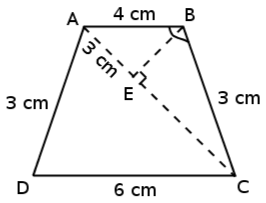
\includegraphics[width=200px]{col11306.imgs/m39408_q1trig.png} % ;q1trig.png;;;6.0;8.5;
      \vspace{2pt}
    \vspace{.1in}
    \end{center}
 \end{figure}       \item We will use triangle ABE and triangle BEC to get the two angles, and then we will add these two angles together to find the angle we want.\item We use sin for both triangles since we have the hypotenuse and the opposite side.\item In triangle ABE we find:
\label{m39408*eid824}\nopagebreak\noindent{}
    \begin{equation}
    \begin{array}{ccc}\hfill sin\left(A\hat{B}E\right)& =& \frac{\mathrm{opp}}{\mathrm{hyp}}\hfill \\ \hfill sin\left(A\hat{B}E\right)& =& \frac{3}{4}\hfill \\ A\hat{B}E& =& {sin}^{-1}\left(\frac{3}{4}\right)\hfill \\ A\hat{B}E& =& {48,59}^{\circ }\hfill \end{array}\tag{14.18}
      \end{equation}
We use the theorem of Pythagoras to find $\mathrm{EC}=4,4\phantom{\rule{1pt}{0ex}}\mathrm{cm}$.
In triangle BEC we find:
\label{m39408*eid82344}\nopagebreak\noindent{}
    \begin{equation}
    \begin{array}{ccc}\hfill sin\left(C\hat{B}E\right)& =& \frac{\mathrm{opp}}{\mathrm{hyp}}\hfill \\ \hfill sin\left(C\hat{B}E\right)& =& \frac{4,4}{5}\hfill \\ A\hat{B}E& =& {sin}^{-1}\left(\frac{4,4}{5}\right)\hfill \\ C\hat{B}E& =& {61,64}^{\circ }\hfill \end{array}\tag{14.19}
      \end{equation}
\item We add the two angles together to get: ${48,59}^{\circ }+{61,64}^{\circ }={110,23}^{\circ }$\end{enumerate}
    \end{exercise}
    \end{mdframed}
    }
    \noindent
  \label{m39408**end}
%          \section{ The trig functions for any angle and applications}
%     \nopagebreak
%             \label{m39411} $ \hspace{-5pt}\begin{array}{cccccccccccc}   
\includegraphics[width=0.75cm]{col11306.imgs/summary_fullmarks.png} &   \end{array} $ \hspace{2 pt}\raisebox{-5 pt}{} {(section shortcode: MG10104 )} \par 
%     
%     
%     
% 	\par
%       \label{m39411*cid6}
%             \subsection{ Simple Applications of Trigonometric Functions}
%             \nopagebreak
%             
       \label{m39411*uid25}
            \subsection{ Height and Depth}
            \nopagebreak
    \setcounter{subfigure}{0}
	\begin{figure}[H] % horizontal\label{m39411*uid26}
    \begin{center}
    \rule[.1in]{\figurerulewidth}{.005in} \\
        \label{m39411*uid26!!!underscore!!!media}\label{m39411*uid26!!!underscore!!!printimage}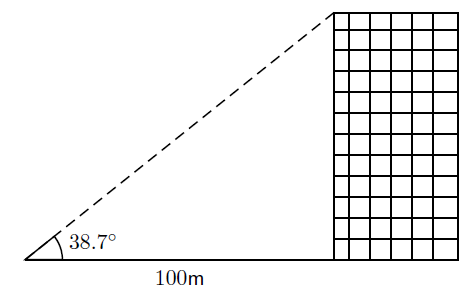
\includegraphics[width=300px]{col11306.imgs/m39411_MG10C15_012.png} % m39411;MG10C15\_012.png;;;6.0;8.5;
      \vspace{2pt}
    \vspace{\rubberspace}\par \begin{cnxcaption}
	  \small \textbf{Figure 14.18: }Determining the height of a building using trigonometry.
	\end{cnxcaption}
    \vspace{.1in}
    \rule[.1in]{\figurerulewidth}{.005in} \\
    \end{center}
 \end{figure}       
        \label{m39411*id81653}One simple task is to find the height of a building by using trigonometry. We could just use a tape measure lowered from the roof, but this is impractical (and dangerous) for tall buildings. It is much more sensible to measure a distance along the ground and use trigonometry to find the height of the building.\par 
        \label{m39411*id81658}Figure~14.18 shows a building whose height we do not know. We have walked 100~m away from the building and measured the angle from the ground up to the top of the building. This angle is found to be $38,{7}^{\circ }$. We call this angle the \textsl{angle of elevation}. As you can see from Figure~14.18, we now have a right-angled triangle. As we know the length of one side and an angle, we can calculate the height of the triangle, which is the height of the building we are trying to find.\par 
        \label{m39411*id81702}If we examine the figure, we see that we have the \textsl{opposite} and the \textsl{adjacent} of the angle of elevation and we can write:\par 
        \label{m39411*id81717}\nopagebreak\noindent{}
    \begin{equation}
    \begin{array}{ccc}\hfill tan38,{7}^{\circ }& =& \frac{\mathrm{opposite}}{\mathrm{adjacent}}\hfill \\ & =& \frac{\mathrm{height}}{100\phantom{\rule{0.166667em}{0ex}}\mathrm{m}}\hfill \\ \hfill \mathrm{height}& =& 100\phantom{\rule{0.166667em}{0ex}}\mathrm{m}\ensuremath{\times}tan38,{7}^{\circ }\hfill \\ & =& 80\phantom{\rule{0.166667em}{0ex}}\mathrm{m}\hfill \end{array}\tag{14.25}
      \end{equation}
\par
            \label{m39411*secfhsst!!!underscore!!!id1381}\vspace{.5cm} 
      \noindent
      \hspace*{-30pt}
\includegraphics[width=0.5in]{col11306.imgs/pspencil2.png}   \raisebox{25mm}{   
      \begin{mdframed}[linewidth=4, leftmargin=40, rightmargin=40]  
      \begin{exercise}
    \noindent\textbf{Exercise 14.6:  Height of a tower }
        \label{m39411*probfhsst!!!underscore!!!id1382}
        \label{m39411*id81869}A block of flats is 100m away from a cellphone tower. Someone stands at $B$. They measure the angle from $B$ up to the top of the tower $E$ to be 62 ${}^{\circ }$. This is the angle of elevation. They then measure the angle from $B$ down to the bottom of the tower at $C$ to be 34 ${}^{\circ }$. This is the angle of depression.What is the height of the cellph one tower correct to 1 decimal place?\par 
        \label{m39411*id81948}
    \setcounter{subfigure}{0}
	\begin{figure}[H] % horizontal\label{m39411*id81949}
    \begin{center}
    \label{m39411*id81949!!!underscore!!!media}\label{m39411*id81949!!!underscore!!!printimage}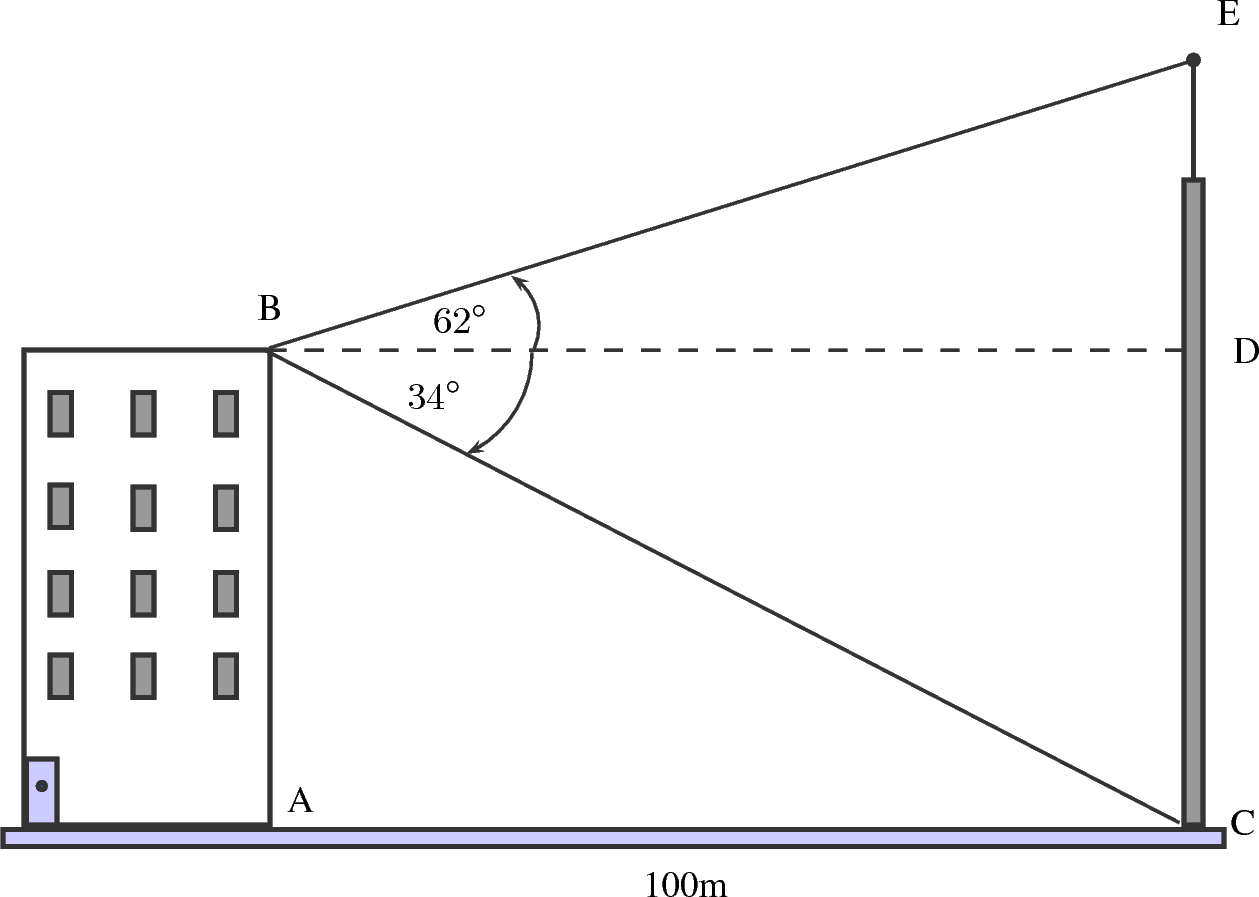
\includegraphics{col11306.imgs/m39411_MG10C15_013.png} % m39411;MG10C15\_013.png;;;6.0;8.5;
      \vspace{2pt}
    \vspace{.1in}
    \end{center}
 \end{figure}       
        \par 
        \vspace{5pt}
        \label{m39411*solfhsst!!!underscore!!!id1394}\noindent\textbf{Solution to Exercise } \label{m39411*listfhsst!!!underscore!!!id1394}\begin{enumerate}[noitemsep, label=\textbf{Step} \textbf{\arabic*}. ] 
            \leftskip=20pt\rightskip=\leftskip\item  
        \label{m39411*id81976}To find the height of the tower, all we have to do is find the length of $CD$ and $DE$. We see that $▵BDE$ and $▵BDC$ are both right-angled triangles. For each of the triangles, we have an angle and we have the length $AD$. Thus we can calculate the sides of the triangles.\par 
        \item  
        \label{m39411*id82067}We are given that the length $AC$ is 100m. $CABD$ is a rectangle so $BD\phantom{\rule{4pt}{0ex}}=\phantom{\rule{4pt}{0ex}}AC\phantom{\rule{4pt}{0ex}}=\phantom{\rule{4pt}{0ex}}100\mathrm{m}$.\par 
        \label{m39411*id82138}\nopagebreak\noindent{}
          
    \begin{equation}
    \begin{array}{ccc}\hfill tan\left(C\hat{B}D\right)& =& \frac{CD}{BD}\hfill \\ \hfill \ensuremath{\Rightarrow}\phantom{\rule{4pt}{0ex}}\phantom{\rule{4pt}{0ex}}\phantom{\rule{4pt}{0ex}}\phantom{\rule{4pt}{0ex}}CD& =& BD\ensuremath{\times}tan\left(C\hat{B}D\right)\hfill \\ & =& 100\ensuremath{\times}tan{34}^{\circ }\hfill \end{array}\tag{14.26}
      \end{equation}
        \label{m39411*id82283}Use your calculator to find that $tan{34}^{\circ }=0,6745$. Using this, we find that $CD=67,45$m\par 
        \item  
        \label{m39411*id82354}\nopagebreak\noindent{}
          
    \begin{equation}
    \begin{array}{ccc}\hfill tan\left(D\hat{B}E\right)& =& \frac{DE}{BD}\hfill \\ \hfill \ensuremath{\Rightarrow}\phantom{\rule{4pt}{0ex}}\phantom{\rule{4pt}{0ex}}\phantom{\rule{4pt}{0ex}}\phantom{\rule{4pt}{0ex}}DE& =& BD\ensuremath{\times}tan\left(D\hat{B}E\right)\hfill \\ & =& 100\ensuremath{\times}tan{62}^{\circ }\hfill \\ & =& 188,07\phantom{\rule{0.166667em}{0ex}}\mathrm{m}\hfill \end{array}\tag{14.27}
      \end{equation}
        \item  
        \label{m39411*id82527}We have that the height of the tower
$CE=CD+DE=67,45\phantom{\rule{0.166667em}{0ex}}\mathrm{m}+188,07\phantom{\rule{0.166667em}{0ex}}\mathrm{m}=255.5\phantom{\rule{0.166667em}{0ex}}\mathrm{m}$.
 \par 
        \end{enumerate}
    \end{exercise}
    \end{mdframed}
    }
    \noindent
      \label{m39411*uid27}
            \subsection{ Maps and Plans}
            \nopagebreak
        \label{m39411*id82626}Maps and plans are usually scale drawings. This means that they are an exact copy of the real thing, but are usually smaller. So, only lengths are changed, but all angles are the same. We can use this idea to make use of maps and plans by adding information from the real world.\par 
\label{m39411*secfhsst!!!underscore!!!id1596}\vspace{.5cm} 
      \noindent
      \hspace*{-30pt}
\includegraphics[width=0.5in]{col11306.imgs/pspencil2.png}   \raisebox{25mm}{   
      \begin{mdframed}[linewidth=4, leftmargin=40, rightmargin=40]  
      \begin{exercise}
    \noindent\textbf{Exercise 14.7:  Scale Drawing }
        \label{m39411*probfhsst!!!underscore!!!id1597}
        \label{m39411*id82645}A ship approaching Cape Town Harbour reaches point A on the map, due south of Pretoria and due east of Cape Town. If the distance from Cape Town to Pretoria is 1000km, use trigonometry to find out how far east the ship is from Cape Town, and hence find the scale of the map.\par 
        \label{m39411*id82652}
    \setcounter{subfigure}{0}
	\begin{figure}[H] % horizontal\label{m39411*id82657}
    \begin{center}
    \label{m39411*id82657!!!underscore!!!media}\label{m39411*id82657!!!underscore!!!printimage}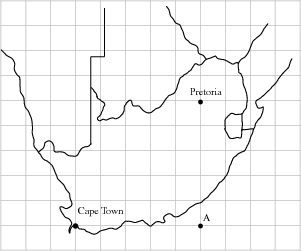
\includegraphics[width=300px]{col11306.imgs/m39411_MG10C15_014.png} % m39411;MG10C15\_014.png;;;6.0;8.5;
      \vspace{2pt}
    \vspace{.1in}
    \end{center}
 \end{figure}       
        \par 
        \vspace{5pt}
        \label{m39411*solfhsst!!!underscore!!!id1611}\noindent\textbf{Solution to Exercise } \label{m39411*listfhsst!!!underscore!!!id1611}\begin{enumerate}[noitemsep, label=\textbf{Step} \textbf{\arabic*}. ] 
            \leftskip=20pt\rightskip=\leftskip\item  
        \label{m39411*id82688}We already know the distance between Cape Town and $A$ in blocks from the given map (it is 5 blocks). Thus if we work out how many kilometers this same distance is, we can calculate how many kilometers each block represents, and thus we have the scale of the map.\par 
        \item  
        \label{m39411*id82707}Let us denote Cape Town with $C$ and Pretoria with $P$.
We can see that triangle $APC$ is a right-angled triangle. Furthermore, we see that the distance $AC$ and distance $AP$ are both 5 blocks. Thus it is an isoceles triangle, and so $A\hat{C}P=A\hat{P}C={45}^{\circ }$.\par 
        \item  
        \label{m39411*id82816}\nopagebreak\noindent{}
          
    \begin{equation}
    \begin{array}{cc}\hfill CA=& CP\ensuremath{\times}cos\left(A\hat{C}P\right)\\ \hfill =& 1000\ensuremath{\times}cos\left({45}^{\circ }\right)\\ \hfill =& \frac{1000}{\sqrt{2}}\phantom{\rule{0.166667em}{0ex}}\mathrm{km}\end{array}\tag{14.28}
      \end{equation}
        \label{m39411*id82923}To work out the scale, we see that\par 
        \label{m39411*id82929}\nopagebreak\noindent{}
          
    \begin{equation}
    \begin{array}{cc}\hfill 5\phantom{\rule{4pt}{0ex}}\text{blocks}=& \frac{1000}{\sqrt{2}}\phantom{\rule{0.166667em}{0ex}}\text{km}\\ \hfill \ensuremath{\Rightarrow}\phantom{\rule{4pt}{0ex}}\phantom{\rule{4pt}{0ex}}\phantom{\rule{4pt}{0ex}}\phantom{\rule{4pt}{0ex}}\phantom{\rule{4pt}{0ex}}\phantom{\rule{4pt}{0ex}}1\phantom{\rule{4pt}{0ex}}\text{block}=& \frac{200}{\sqrt{2}}\phantom{\rule{0.166667em}{0ex}}\text{km}\end{array}\tag{14.29}
      \end{equation}
        \end{enumerate}
    \end{exercise}
    \end{mdframed}
    }
    \noindent
\par
            \label{m39411*secfhsst!!!underscore!!!id1745}\vspace{.5cm} 
      \noindent
      \hspace*{-30pt}
\includegraphics[width=0.5in]{col11306.imgs/pspencil2.png}   \raisebox{25mm}{   
      \begin{mdframed}[linewidth=4, leftmargin=40, rightmargin=40]  
      \begin{exercise}
    \noindent\textbf{Exercise 14.8:  Building plan }
        \label{m39411*probfhsst!!!underscore!!!id1746}
        \label{m39411*id83053}Mr Nkosi has a garage at his house, and he decides that he wants to add a corrugated iron roof to the side of the garage. The garage is 4m high, and his sheet for the roof is 5m long. If he wants the roof to be at an angle of ${5}^{\circ }$, how high must he build the wall $BD$, which is holding up the roof? Give the answer to 2 decimal places.\par 
        \label{m39411*id83089}
    \setcounter{subfigure}{0}
	\begin{figure}[H] % horizontal\label{m39411*id83090}
    \begin{center}
    \label{m39411*id83090!!!underscore!!!media}\label{m39411*id83090!!!underscore!!!printimage}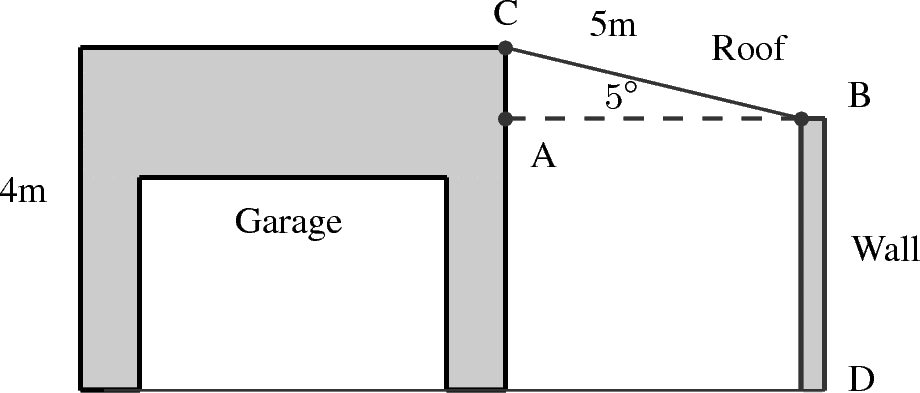
\includegraphics{col11306.imgs/m39411_MG10C15_015.png} % m39411;MG10C15\_015.png;;;6.0;8.5;
      \vspace{2pt}
    \vspace{.1in}
    \end{center}
 \end{figure}       
        \par 
        \vspace{5pt}
        \label{m39411*solfhsst!!!underscore!!!id1758}\noindent\textbf{Solution to Exercise } \label{m39411*listfhsst!!!underscore!!!id1758}\begin{enumerate}[noitemsep, label=\textbf{Step} \textbf{\arabic*}. ] 
            \leftskip=20pt\rightskip=\leftskip\item  
        \label{m39411*id83116}We see that the triangle $ABC$ is a right-angled triangle. As we have one side and an angle of this triangle, we can calculate $AC$. The height of the wall is then the height of the garage minus $AC$.\par 
        \item  
        \label{m39411*id83164}If $BC$=5m, and angle $A\hat{B}C={5}^{\circ }$, then\par 
        \label{m39411*id83209}\nopagebreak\noindent{}
          
    \begin{equation}
    \begin{array}{ccc}\hfill AC& =& BC\ensuremath{\times}sin\left(A\hat{B}C\right)\hfill \\ & =& 5\ensuremath{\times}sin{5}^{\circ }\hfill \\ & =& 5\ensuremath{\times}0,0871\hfill \\ & =& 0.4358\phantom{\rule{0.166667em}{0ex}}\mathrm{m}\hfill \end{array}\tag{14.30}
      \end{equation}
        \label{m39411*id83338}Thus we have that the height of the wall $BD=4\phantom{\rule{0.166667em}{0ex}}\mathrm{m}-0.4358\phantom{\rule{0.166667em}{0ex}}\mathrm{m}=3.56\phantom{\rule{0.166667em}{0ex}}\mathrm{m}$.
 \par 
        \end{enumerate}
    \end{exercise}
    \end{mdframed}
    }
    \noindent
\label{m39411*secfhsst!!!underscore!!!id1847}
            \subsection{ Exercise: Applications of Trigonometric Functions }
            \nopagebreak
        \label{m39411*id83420}\begin{enumerate}[noitemsep, label=\textbf{\arabic*}. ] 
            \label{m39411*uid28}\item A boy flying a kite is standing 30~m from a point directly under the
kite. If the string to the kite is 50~m long, find the angle of
elevation of the kite.\newline
\label{m39411*uid29}\item What is the angle of elevation of the sun when a tree 7,15 m tall
casts a shadow 10,1 m long?\newline
\end{enumerate}
  \label{m39411**end}
\par \raisebox{-5 pt}{
\includegraphics[width=0.5cm]{col11306.imgs/summary_www.png}} Find the answers with the shortcodes:
 \par \begin{tabular}[h]{cccccc}
 (1.) lcY  &  (2.) lcr  & \end{tabular}
% 
%          \section{ Graphs of trig functions}
%     \nopagebreak
%             \label{m39414} $ \hspace{-5pt}\begin{array}{cccccccccccc}   
\includegraphics[width=0.75cm]{col11306.imgs/summary_video.png} &   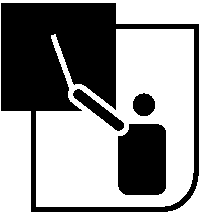
\includegraphics[width=0.75cm]{col11306.imgs/summary_presentation.png} &   \end{array} $ \hspace{2 pt}\raisebox{-5 pt}{} {(section shortcode: MG10105 )} \par 
%     
%     
%     
            \section{ Summary}
            \nopagebreak
            \label{m39414*eip-197}\begin{itemize}[noitemsep]
            \item We can define three trigonometric functions for right angled triangles: sine (sin), cosine (cos) and tangent (tan).\item Each of these functions have a reciprocal: cosecant (cosec), secant (sec) and cotangent (cot).
\item We can use the principles of solving equations and the trigonometric functions to help us solve simple trigonometric equations.\item We can solve problems in two dimensions that involve right angled triangles.\item For some special angles, we can easily find the values of sin, cos and tan.\item We can extend the definitions of the trigonometric functions to any angle.\item 
Trigonometry is used to help us solve problems in 2-dimensions, such as finding the height of a building.\item 
We can draw graphs for sin, cos and tan\end{itemize}
        \label{m39414*cid8}
            \section{ End of Chapter Exercises}
            \nopagebreak
      \label{m39414*id92202}\begin{enumerate}[noitemsep, label=\textbf{\arabic*}. ] 
            \label{m39414*uid98}\item Calculate the unknown lengths
    \setcounter{subfigure}{0}
	\begin{figure}[H] % horizontal\label{m39414*id92222}
    \begin{center}
    \label{m39414*id92222!!!underscore!!!media}\label{m39414*id92222!!!underscore!!!printimage}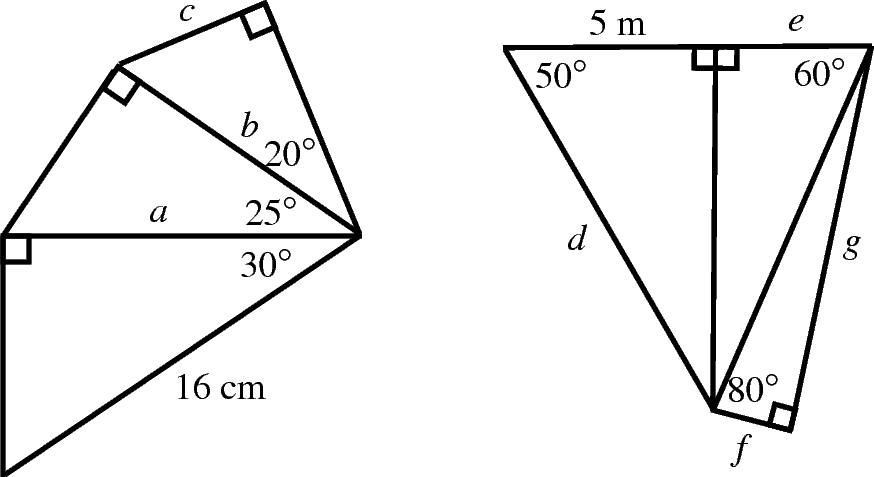
\includegraphics{col11306.imgs/m39414_MG10C15_041.png} % m39414;MG10C15\_041.png;;;6.0;8.5;
      \vspace{2pt}
    \vspace{.1in}
    \end{center}
 \end{figure}               \label{m39414*uid99}\item In the triangle $PQR$, $PR=20$~cm, $QR=22$~cm and $P\hat{R}Q={30}^{\circ }$. The perpendicular line from $P$ to $QR$ intersects $QR$ at $X$. Calculate
\label{m39414*id92364}\begin{enumerate}[noitemsep, label=\textbf{\alph*}. ] 
            \label{m39414*uid100}\item the length $XR$,
\label{m39414*uid101}\item the length $PX$, and
\label{m39414*uid102}\item the angle $Q\hat{P}X$\end{enumerate}
                \label{m39414*uid103}\item A ladder of length 15 m is resting against a wall, the base of the ladder is 5 m from the wall. Find the angle between the wall and the ladder?\newline
\label{m39414*uid104}\item A ladder of length 25 m is resting against a wall, the ladder makes an angle ${37}^{\circ }$ to the wall. Find the distance between the wall and the base of the ladder?\newline
\label{m39414*uid105}\item In the following triangle find the angle $A\hat{B}C$
    \setcounter{subfigure}{0}
	\begin{figure}[H] % horizontal\label{m39414*id92525}
    \begin{center}
    \label{m39414*id92525!!!underscore!!!media}\label{m39414*id92525!!!underscore!!!printimage}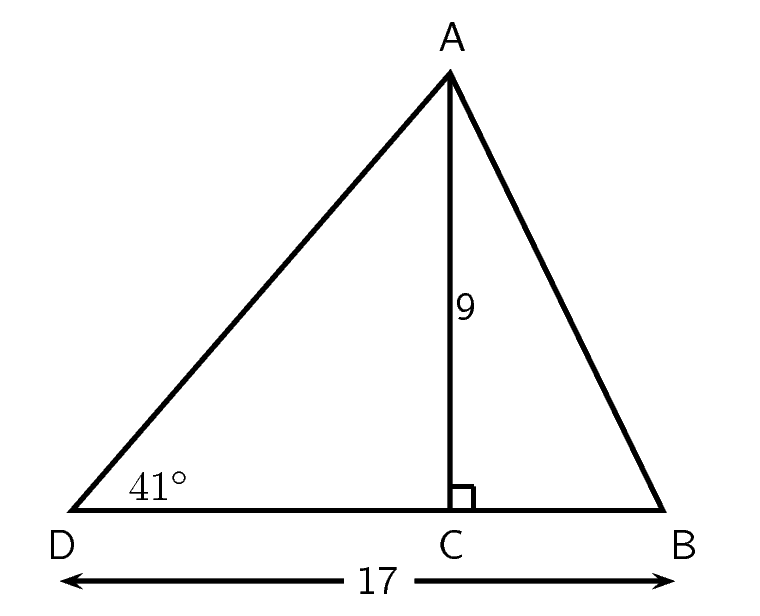
\includegraphics{col11306.imgs/m39414_MG10C15_042.png} % m39414;MG10C15\_042.png;;;6.0;8.5;
      \vspace{2pt}
    \vspace{.1in}
    \end{center}
 \end{figure}               \label{m39414*uid106}\item In the following triangle find the length of side $CD$
    \setcounter{subfigure}{0}
	\begin{figure}[H] % horizontal\label{m39414*id92559}
    \begin{center}
    \label{m39414*id92559!!!underscore!!!media}\label{m39414*id92559!!!underscore!!!printimage}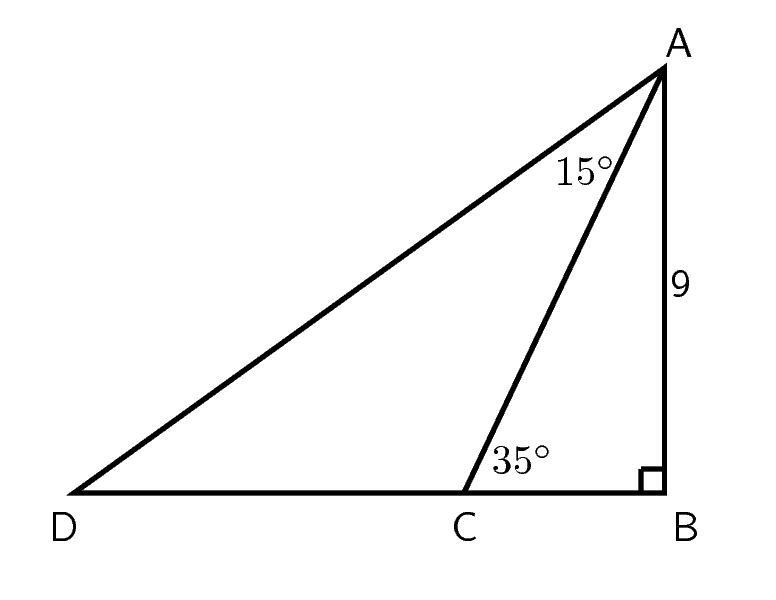
\includegraphics{col11306.imgs/m39414_MG10C15_043.png} % m39414;MG10C15\_043.png;;;6.0;8.5;
      \vspace{2pt}
    \vspace{.1in}
    \end{center}
 \end{figure}               \label{m39414*uid107}\item $A\left(5;0\right)$ and $B\left(11;4\right)$. Find the angle between the line through A and B and the x-axis.\newline
\label{m39414*uid108}\item $C\left(0;-13\right)$ and $D\left(-12;14\right)$. Find the angle between the line through C and D and the y-axis.\newline
\label{m39414*uid110}\item A $5\phantom{\rule{0.166667em}{0ex}}\mathrm{m}$ ladder is placed $2\phantom{\rule{0.166667em}{0ex}}\mathrm{m}$ from the wall. What is the angle the ladder makes with the wall?\newline
\label{m39414*uid981203}\item Given the points: E(5;0), F(6;2) and G(8;-2), find angle $F\hat{E}G$.\newline
            \label{m39414*uid111}\item An isosceles triangle has sides $9\phantom{\rule{0.166667em}{0ex}}\mathrm{cm},\phantom{\rule{0.166667em}{0ex}}9\phantom{\rule{0.166667em}{0ex}}\mathrm{cm}$ and $2\phantom{\rule{0.166667em}{0ex}}\mathrm{cm}$. Find the size of the smallest angle of the triangle.\newline
\label{m39414*uid112}\item A right-angled triangle has hypotenuse $13\phantom{\rule{0.166667em}{0ex}}\mathrm{mm}$. Find the length of the other two sides if one of the angles of the triangle is ${50}^{\circ }$.\newline
\label{m39414*uid113}\item One of the angles of a rhombus (\textbf{rhombus} - A four-sided polygon, each of whose sides is of equal length) with perimeter $20\phantom{\rule{0.166667em}{0ex}}\mathrm{cm}$ is ${30}^{\circ }$.
\label{m39414*id92966}\begin{enumerate}[noitemsep, label=\textbf{\alph*}. ] 
            \label{m39414*uid114}\item Find the sides of the rhombus.
\label{m39414*uid115}\item Find the length of both diagonals.
\end{enumerate}
                \label{m39414*uid116}\item Captain Hook was sailing towards a lighthouse with a height of $10\phantom{\rule{0.166667em}{0ex}}\mathrm{m}$.
\label{m39414*id93025}\begin{enumerate}[noitemsep, label=\textbf{\alph*}. ] 
            \label{m39414*uid117}\item If the top of the lighthouse is $30\phantom{\rule{0.166667em}{0ex}}\mathrm{m}$ away, what is the angle of elevation of the boat to the nearest integer?
\label{m39414*uid118}\item If the boat moves another $7\phantom{\rule{0.166667em}{0ex}}\mathrm{m}$ towards the lighthouse, what is the new angle of elevation of the boat to the nearest integer?
\end{enumerate}
                \label{m39414*uid119}\item (Tricky) A triangle with angles ${40}^{\circ },\phantom{\rule{0.166667em}{0ex}}{40}^{\circ }$ and ${100}^{\circ }$ has a perimeter of $20\phantom{\rule{0.166667em}{0ex}}\mathrm{cm}$. Find the length of each side of the triangle.\newline
\end{enumerate}
  \label{m39414**end}
  \label{fbcda86bdf0258b6e91dcea5caee5b76**end}
\par \raisebox{-5 pt}{
\includegraphics[width=0.5cm]{col11306.imgs/summary_www.png}} Find the answers with the shortcodes:
 \par \begin{tabular}[h]{cccccc}
 (1.) la9  &  (2.) laX  &  (3.) laI  &  (4.) la5  &  (5.) laN  &  (6.) laR  &  (7.) lan  &  (8.) laQ  &  (9.) laU  &  (10.) lap  &  (11.) laV  &  (12.) laP  &  (13.) laE  &  (14.) lam  &  (15.) lay  & \end{tabular}
